\documentclass[conference]{IEEEtran}
%%%%%%%%%%%%%%%%%%%%%%%%%%%%%%%%%%%%%%%%%%%%%%%%%%%%%%%
% This is main.tex, as on 22.04.2021.
% This is an unofficial template for Menelaos-NT(https://www.menelaos-nt.eu/) Research Report template based on [IEEE - Manuscript Templates for Conference Proceedings](https://www.ieee.org/conferences/publishing/templates.html) by Michael Shell.
% A modification was made by Zhouyan Qiu.
% Manual: IEEEtran_HOWTO.pdf
%%%%%%%%%%%%%%%%%%%%%%%%%%%%%%%%%%%%%%%%%%%%%%%%%%%%%%%

\IEEEoverridecommandlockouts
% The preceding line is only needed to identify funding in the first footnote. If that is unneeded, please comment it out.
\usepackage{cite}
\usepackage{amsmath,amssymb,amsfonts}
\usepackage{algorithmic}
\usepackage{graphicx}
\usepackage{textcomp}
\usepackage{xcolor}
\usepackage{fancyhdr}
\usepackage{lipsum}% generate text for the example
\usepackage{hyperref}
\usepackage{float} 
\usepackage{pdfpages}

\def\BibTeX{{\rm B\kern-.05em{\sc i\kern-.025em b}\kern-.08em
    T\kern-.1667em\lower.7ex\hbox{E}\kern-.125emX}}
    


\pagestyle{empty}

\begin{document}
\title{Bridging the Data Gap: A Conversational Chatbot Approach to Optimizing Mobile Plan Selection Through HCI Principles}

\author{\IEEEauthorblockN{David Carciente - 40247907}
\IEEEauthorblockA{\textit{Concordia University} \\
Montreal, Canada \\
davidcarciente@outlook.com}
\and
\IEEEauthorblockN{Brian Tkatch - 40191139}
\IEEEauthorblockA{\textit{Concordia University} \\
Montreal, Canada \\
brian@briantkatch.com}
}

\maketitle

\begin{abstract}
This paper investigates how an on-boarding chatbot can bridge the gap between users' actual data requirements and available mobile plans. Through rigorous application of HCI/UX/UI principles and a five-iteration development process, we demonstrate that a conversational interface can significantly improve mobile plan recommendations. Statistical analysis shows our approach achieved 75.2\% greater accuracy than traditional tier-based systems (p = 0.017) and 41.4\% improvement over users' current plans. Usability testing revealed unanimous preference for the chatbot method, with participants reporting reduced cognitive load and increased decision confidence. The research validates that by translating technical specifications into natural language within a carefully designed interface, telecommunications providers can transform the traditionally confusing mobile plan selection process into one that aligns with users' actual needs. This approach not only improves recommendation accuracy but also enhances overall user experience, potentially increasing customer satisfaction while optimizing plan selection.
\end{abstract}

%\thispagestyle{firstpagefooter}

\section{Introduction}
The internet is continuously expanding with numerous services that help humans accomplish their daily tasks and fulfill
various needs. However, accessing the internet from anywhere
and at any time comes at a cost. Recognizing that individuals
have varying data requirements; telecommunication companies
typically offer multiple tiers of bandwidth. This means not
all users require access to the same amount of data. Given
these varying needs, telecommunication companies present
different plans, often summarized in feature matrices. These
matrices provide high-level details, such as bandwidth, speed,
and cost. However, there’s often no clear correlation between
these attributes and actual user usage, leading to confusion.
This raises an important question:\begin{quote}
    How much data does a user genuinely need to
accomplish their daily goals on the internet?
\end{quote}
\subsection{Hypothesis}
Ensuring mobile phone plans accurately align with users’
actual data needs is essential for a positive purchasing experience. Mismatched plans, where users pay for too much
or too little data, often lead to dissatisfaction. This paper
hypothesizes that an on-boarding chatbot can effectively gather
user insights, bridging the gap between users’ real data requirements and the available plans, thus recommending the optimal
data plan.

\subsection{Project Goals and Scope}
The goal of this paper is to evaluate the hypothesis and user requirements derived in the previous report of SOEN 357 course. This is done by designing a prototype, and continuously evaluating the design with user feedback to then disprove the null hypothesis. 

\subsubsection{User Requirements (8)}
\begin{enumerate}
    \item The user’s decision of a mobile plan should not be stressful or confusing.
    \item The user’s mobile plan’s service fees should be clearly presented and explained to the user.
    \item The user should be able to select their preferred mobile carrier.
    \item The user should be informed of the data plan in terms of their usability goals in natural language, not just their technical bandwidth.
    \item The user should be informed about the value from the cost of the plan.
    \item The user should be able to be informed about the differences between higher or lower tiered plans.
    \item The user should be able to compare their carrier’s plan with other carriers.
    \item The user should use an interface when selecting their phone plan, that follows a standardized format to reduce cognitive overload.
\end{enumerate}
\section{Related Work}
As of this report, there has not been any new research related to the discussion of the Chatbot itself and the hypothesis, as they have all been derived to satisfy the user requirements from the previous report. However, there will be discussions in the next section related to methods used in UI/UX/HCI.
\section{Methods}
\subsection{Research Methods}
\subsubsection{Double Diamond Process}
The Designs Council’s Double Diamond process is a method which provides a systematic approach to interaction Design (IxD). In the previous report, the first \textit{diamond}, or phase was completed, which is to determine the requirements. In this report, the 2nd diamond will be used, which suggests to "develop potential solution and deliver solutions that work". The process used will be used incrementally, which will allow for rapid changes depending on the user's needs.
\subsubsection{The Spiral Process}
As mentioned in the double diamond process, there is a need to develop functional solutions. This could include many variations, but a single working solution should be chosen as the final result. In the scope of this paper, a prototype will be proposed as a final solution. 

The spiral process comes in for facilitating the process of designing a user interface. It embraces change, and promotes iterative refinement through continual user feedback. This is a key method used, as the more feedback we get, the more we converge on the ideal design.
\subsection{User Interface Design Methods}
This section is heavily based on the designed flow of a chatbot, designed in the previous report. It has been attached in the appendix as a reference. High level discussions of the required UI elements will be mentioned first, then in Implementation Methods will provide concrete technical tools based off the UI/UX/HCI research. The solutions will be presented in the results section.
\subsubsection{User Design Elements}
According to the designed user flow, there will contain at least 6 different interfaces. This includes:
\begin{itemize}
  \item \textbf{Home Page}: A page where the user accesses the website.
  \item \textbf{Chatbot Interface}: A subset of the page which contains a Chatbot that a user can interact with.
  \item \textbf{User Needs}: A page that contains information about the User Needs.
  \item \textbf{Desired Plan}: A page that contains information about the user's ideal plan.
  \item \textbf{Hidden Fees}: A page that contains information about the phone plan's hidden fees.
  \item \textbf{Summary of Plan}: A digestive summary of the last three points (User Needs, Desired Plan, Hidden Fees)
\end{itemize}
This list reveals a lot of information that will be required:
\begin{itemize}
    \item \textbf{Cards} can be used to display grouped information about the interface. This can also allow to reduce the likelihood of the interface needing to be scrollable. Having everything in one page will make the design clear. 
    \item The interface for the chatbot (as discussed in the previous report) will require a \textbf{text-field} which the user can provide information, and a \textbf{button} to submit their message or a keyboard shortcut. An expected response is required via a \textbf{text-box} message.
    \item Between the User Needs, Desired Plan, Hidden Fees and Summary of Plan, they will be presented in a sequential order. Hence, \textbf{breadcrums} will be used in order to give context to the user on how close they are in figuring out their plan. 
    \item For each result after using the chatbot, should be presented via a \textbf{Bento Menu} \cite{CareerFoundryUI}. Since cards will be used as a primary basis to displaying information, the Bento menu can be alternated with the \textit{Meatball} and \textit{Kebab}. 
\end{itemize}
% \begin{description}
%   \item[First:] \textbf{Home Page}: A page where the user accesses the website.
%   \item[Second:] \textbf{Chatbot Interface}: A subset of the page which contains a Chatbot that a user can interact with.
%   \item[Third:] \textbf{User Needs}: A page that contains information about the User Needs.
%   \item[Fourth:] \textbf{Desired Plan}: A page that contains information about the user's ideal plan.
%   \item[Fifth:] \textbf{Hidden Fees}: A page that contains information about the phone plan's hidden fees.
%   \item[Sixth:] \textbf{Summary of Plan}: A digest of the last three points (User Needs, Desired Plan, Hidden Fees)
% \end{description}


\subsubsection{6 Pillars of UI Design}
On top of basic design elements, there should be a guideline in how to organize the information, from the perspective of a user's limitations \cite{Sommerville1996}.

\begin{itemize}
    \item \textbf{User Familiarity}: The application should relate to familiar concepts. This will be accomplished using a Chatbot which provides a conversation similar to the interface of a regular messaging service. In addition, the current phone plan process is somewhat a familiar one. Reinventing the way that the information is presented is not a good practice, as it may cause confusion. The goal is to have a common golden mean between usability and familiarity.
    \item \textbf{Consistency}: The interface should be consistent between pages. This will be considered heavily when introducing the needs of the user and their phone plans. However, using inconsistencies can be very useful when comparing between different phone plans, which can help bring the user's attention.
    \item \textbf{Least Surprise}: The UI should be designed to not surprise the users, and be as obvious as possible. In other words, all UI elements intentions should be understood by the user.
    \item \textbf{Recoverability}: This is when the user has the ability to make mistakes, and allow them to recover, to avoid disrupting the flow to reaching their goals. In this case, the only source of input comes from the Chatbot, hence, the user can make mistakes when inserting data into the bot. 
    \item \textbf{User assistance}: While the user is trying to understand their phone usage and desired plan, they should have a clear guide on how to reach it. A guide on the entry point of the interface can be beneficial to explain how to use the service. 
    \item \textbf{User diversity}: The interface should be easily understood and accessible by everyone. This is very important, as the hypothesis targets users of all ages and different technical backgrounds. Hence, it needs to be accessible to them.
\end{itemize}
\subsubsection{Cognition}
Cognition is an important aspect of designing an interface, as the diversity of users for this interface is varied. The cognitive process encapsulates: Fluency, Attention, Perception, Memory, Learning, Reading, Speaking, Listening, Problem solving, planning, reasoning and decision making. This section will discuss how these factors will take into account for designing the perfect interface.
\begin{itemize}
    \item \textbf{Cognitive Fluency}: When the user will use the interface, they should have to use the least amount of thinking possible. This is backed up by our user requirements. In the scope of the interface, when the chatbot asks questions, they should be as simple as possible. In addition, there should be a strong reduction in explaining the phone plan to the user. 
    
    One key aspect is using familiarity. In other words, the user should not have to put effort into understanding what a gigabyte is, but more knowing what they do during the day. It is very easy to recall what a user's habits are, in contrast to knowing how much mobile data they utilize. Using Jakob's law, by incorporating similar design styles like other interfaces, such as the user design elements mentioned earlier, will help design the most effective. 
    
    Some key examples of having strong cognitive fluency, is to focus on typography, excellent spacing between cards and ui elements, colours, and the content itself.
    \begin{itemize}
        \item \textbf{Typography}: The typography that will be chosen is called \textbf{Inter}. Designed by Rasmus Andersson, the topography has a strong emphasis on high readability and excellent clarity in user interfaces \cite{interDesign}.
        \item \textbf{Spacing}: The spacing will follow the principle Bento Menu, as discussed in User Design Elements section. The idea here is that by having good spacing will imply a stronger attention span\cite{Tullis1987}. More discussed in the attention section.
        \item \textbf{Color}: In order to make the color scheme familiar, the interface should follow the colors of the mobile carrier plans. The idea is to have a general color scheme for the application, then using the exact colors to match the chosen mobile carrier. This allows to not only have \textbf{affordances}, but to make sure that the user understands the context they are in, and are not lost or confused. This overall will stimulate different types of memory, which is their mobile carrier they recall.
        
        Another point is picking the right color that is compatible with all cultures. This is because every user has a different world view. This is why the blue palette will be chosen as the overall theme of the application. Blue represents calm, trust, evokes spirituality and strength. This will then lead to the user being in a good mood, which will cause cognitive fluency.
        \item \textbf{Content}: The content itself will contain as mentioned in each section of the design flow. However, the way it is presented should provide more text than numbers, but not too much text where it overwhelms the user. An example is Hick's law, in which it mentions that we should not present too many elements for choices together. This is in fact the reason why mobile phone plans are already confusing to pick. Hence, there should be a balance uncovered, which can only be found during usability testing. This will also be discussed later in the results.
        
        The content is also based off the conversation of a chatbot. The strategy here is to evoke a \textit{priming effect}. For example, when the chatbot is going to respond to the user, it shouldn't just give the response, but should prime the user by using a typing indicator. This will then influence a stimulus to expect a reply and ready to take action. 
        
    \end{itemize}
    \item \textbf{Attention}: This is an important factor. Since the primary target are mobile phone users, such users are already prone to a limited attention span \cite{Ward2017}. A key solution is to limit the amount of content, and only provide the most minimal amount of information. It is important though to consider the generational gaps, as different generations have different attention spans. Hence, it is important to simply reduce the amount of multi tasking tasks, but have a clear, linear path of what they need to accomplish\cite{Carrier2009MultitaskingAG}. In this case, the user flow accomplishes this, as they are not needed to do more than one task at a time.
    \item \textbf{Perception}:
    The idea behind perception is that every human interprets the world depending on their experiences. Hence, when developing the interface, this must also be considered. The way this will be done is analyzing the \textbf{Law's of Prägnanz}, which are based off Gestalt's visual perception principles of how humans perceive the world. 
    \begin{itemize}
        \item \textbf{Law of Proximity}: The Law of Proximity states that elements placed near one another are perceived as belonging to the same group. This principle supports the organization of interface elements such as grouped usage tiers, plan components, or sets of options presented within a conversational interface. Proximity aids the user in distinguishing between functionally related sections, for example, separating primary and secondary content or aligning question-and-answer pairs within a chatbot interface.
        \item \textbf{Principle of Common Regions}: According to this principle, elements enclosed within a shared visual boundary—such as a background container or bordered area—are perceived as related, regardless of their spacing. This is commonly applied in card-based layouts, where each card encapsulates a distinct concept or option. In interfaces where users must compare multiple plans or recommendations, enclosing each item within a defined region helps clarify boundaries between items while reinforcing group identity.
        \item \textbf{Law of Similarity}: This principle asserts that visually similar elements—sharing characteristics such as color, shape, size, or typography—are likely to be interpreted as part of the same category or function. For example, a uniform appearance across selection options, usage levels, or response messages reinforces consistency and predictability in interaction. Similarity also contributes to the development of visual hierarchies, guiding the user through repeated patterns and familiar structures across different stages of interaction.
        \item \textbf{Law of Closure}: The Law of Closure refers to the tendency of users to perceive incomplete figures or layouts as complete. Designers can leverage this principle to imply structure using alignment and spacing rather than explicitly drawing boundaries. Closure can be effective in progress indicators, breadcrumb navigation, or sequences of steps where the user can mentally complete the pathway without every element being fully rendered.
        \item \textbf{Law of Symmetry}: This principle posits that users are more likely to perceive symmetrical elements as unified and balanced. Interfaces that use symmetrical grids, centralized layouts, or even spacing enhance visual stability and support scannability. This is especially relevant in comparative views, such as when users review multiple plan options presented side by side or assess usage tiers within a unified framework.
        \item \textbf{Law of Common Fate}: Elements that move or change together are interpreted as belonging to the same group. This principle is commonly applied in dynamic interactions, such as when multiple components update simultaneously or are revealed as a unit. In conversational interfaces, sequential or grouped chatbot responses can benefit from synchronized appearance to indicate logical cohesion. Likewise, grouped transitions in recommendation outputs reinforce their relational structure.

        \item \textbf{Law of Continuity}: The Law of Continuity refers to the visual preference for aligned or smoothly flowing elements. Alignment along a linear path creates a sense of continuity and progression. In multi-step processes, such as onboarding flows or sequential navigation from user input to summary, horizontal or vertical alignment can visually reinforce directional movement. This principle supports the structuring of linear processes, aiding users in understanding the order and context of their current position.

        \item \textbf{Law of Past Experience}: This principle emphasizes that interpretation is influenced by a user's prior interactions and learned patterns. Interfaces benefit from incorporating familiar elements—such as chat formats, mobile plan layouts, or brand-related color schemes—that align with common user expectations. Leveraging past experience allows users to engage with the system more effectively, as minimal effort is required to interpret familiar components.

        \item \textbf{Principle of Focal Point}: The focal point principle states that the most visually distinct element within a layout will attract the user’s attention first. Contrast in size, color, or positioning can be used to guide attention to key interface components such as primary actions, recommended choices, or alerts. In plan comparison or chatbot confirmation screens, focal points assist in directing user behavior toward confirmation, selection, or further engagement.
        
        \item \textbf{Principle of Figure / Ground}: This principle refers to the ability to distinguish elements of focus (figure) from the background (ground). Clear separation between interactive content and background space is critical for usability. The use of contrast, shadow, layering, or color blocking ensures that important elements—such as message containers, cards, or selection panels—remain visually distinct and easily scannable, even within densely populated interfaces.
    \end{itemize}
    \item \textbf{Memory}:
Memory plays a big role in how people understand and use websites or apps. Designers think about two types of memory: short-term and long-term. Short-term memory can only hold about 5 to 9 things at once, based on Miller’s Law (1956) \cite{Schneider2011AMM}. If users see too much at once, they might get confused, make mistakes, or leave. To avoid this, it helps to group things into smaller, meaningful chunks. For example, showing 9 items as 3 groups of 3 makes it easier to follow. This is especially useful when users go through steps—like comparing phone plans or checking for hidden fees.

Short-term memory helps us with things we need to remember right now, while long-term memory helps us recognize things we've seen before. It’s usually easier to recognize something than to remember it from scratch. That’s why good designs repeat familiar layouts, use matching colors, or show clear paths like breadcrumb trails. This is especially helpful in chatbots, where being able to look back at what was said earlier or seeing the same visual style makes things feel smoother and more comfortable. In short, using recognition helps people feel confident and also learn better over time.

Hick’s Law says that the more choices people see, or the more complex those choices are, the longer it takes them to decide \cite{Schneider2011AMM}. That’s why good design keeps things simple—only showing what’s needed at the time. This approach is called progressive disclosure, where extra details are revealed step by step. Also, screens shouldn’t show more than 7 to 9 lines or items at once, especially when users have to scroll. If content is long—like phone plan details or FAQs—it’s better to break it into sections using cards or expandable areas. This keeps things easy to scan and avoids overwhelming the user’s short-term memory.


    \item \textbf{Reading and Learning}: In interactive systems, reading helps users learn, but it can be tiring and slow—especially when people just want to explore or move quickly. Long instructions or manuals don’t always work well. That’s why modern apps and websites teach users as they go, by building guidance right into the interaction \cite{Carroll1990Nurnberg}. This works especially well in tools like chatbots or multi-step processes, where users are guided step-by-step without needing to read a lot upfront.

Learning within these interfaces can occur in two forms: intentional and incidental. Intentional learning involves deliberate reading or study—such as referring to documentation—while incidental learning happens organically as users interact with the system. The latter is generally more effective in user-centered design, as it allows knowledge to be acquired contextually and effortlessly. When users answer questions about their needs or compare plan options, they are learning about features and terminology in real-time, without requiring a prior understanding of technical language.

To support this, information should be presented progressively and within context. Rather than overwhelming users with large amounts of text, designers can use conversational prompts, short explanations, and embedded tooltips to reinforce understanding. This not only supports learning-by-doing, as emphasized inthe concept of \textit{learning by doing} \cite{Carroll1990Nurnberg}, but also reduces dependence on memory and lowers cognitive strain. Visual aids, such as cards and summaries, further complement textual information, enabling users to retain and apply knowledge without formal instruction .
    \item \textbf{Speaking:} In the scope of this application, there is no plan in the prototype to allow the user to talk to the chatbot. However, this will be discussed later in terms of the scalability of the application.
    \item \textbf{Listening:} In the scope of this application, there is no plan in the prototype to allow the information to be spoken aloud. However, the interface should provide an ability for a text reader to read out loud the application. More discussed in the limitations of the application in this report.
    \item \textbf{Problem Solving, Planning, Reasoning and Recision Making:} Higher-order cognitive processes such as problem-solving, planning, reasoning, and decision-making play a central role in goal-directed user interactions. These processes fall under the domain of reflective cognition, which involves deliberate thought, evaluation of alternatives, and the use of external tools to support mental operations. In the context of user interface design, these cognitive functions are especially relevant when users must weigh multiple options, interpret trade-offs, or choose between plans with varying levels of complexity. Such tasks require interfaces to structure information in ways that reduce decision fatigue while enhancing clarity and comparative understanding.

\end{itemize}
\subsection{Implementation Methods}
This section covers the scope of how the system was implemented, given the methods of UI/UX/HCI discussed above. 
\subsubsection{Technical Tools}
As mentioned in the previous report, the chatbot chosen will be deterministic, to ensure that there are no hallucinations and that information gathering can be standardized. Hence, the solution was to use an external tool called \textbf{Joonbot}. This tool allows for a deterministic chatbot, that can be integrated in any workflow. In addition, the use of HTML and CSS has been used for the front end, which not only integrates the chatbot seamlessly, but also allows to pass information to our landing page, which provides user insight on their required data plan. The reason for choosing web technologies instead of a standalone application is because web is accessible from any device. In contrast, developing an application comes at the burden of maintaining for many different devices. Hence, our application is scalable for any device accessible to the internet. The back-end uses Javascript, which helps provide decision logic and calculate the required data based off the model. Currently, it is hosted on Github Pages, found on in the \href{https://github.com/briantkatch/357-my-little-chomsky}{GitHub Repository}.
\subsubsection{Maintainability and Scalability}
The overall application is build in such a way that allows the application to be implemented anywhere. Since it is serverless, it doesn't have the overhead in paying for hosting. It has easy accessibility to insert data from any resource, and allowed to be implemented on any website.
\begin{itemize}
    \item \textbf{Users Needs}: This section organizes related information into separate cards, using spacing and layout to clearly group each option. The “Average Usage” card stands out with a different background color, helping to guide attention without adding clutter. The screen keeps the interactive parts visually separate from the background, making it easy to focus on what matters.
\\
Text is kept short and focuses on everyday phone usage, like calling, streaming, or browsing, instead of using technical terms or data measurements. This makes it easier for users to connect with the content. The consistent blue color scheme helps create a feeling of calm and trust, while the breadcrumb at the top marks this screen as step 1 of 4, giving users a clear sense of where they are in the process.
\\
The layout keeps information simple by offering four usage profiles, which makes it easy for users to choose without feeling overwhelmed. This approach follows Miller’s Law by limiting the number of items shown at once, helping users stay focused. The “5 GB” option is highlighted to stand out, guiding attention to the most relevant choice through visual emphasis.
\\
Each option includes clear text that connects data usage to real-life activities, helping users make quick and informed choices. These small, easy decisions—also known as micro-decisions—support a smoother experience. The “Next” button is placed prominently and signals the next step in the process. This creates a clear path forward, making the flow feel natural and helping users stay on track, no matter their level of tech experience or age.
\item \textbf{The Ideal Plan:} This section continues the same design style as the previous screen, using the familiar blue theme and breadcrumb navigation—now showing step 2—to help users feel a sense of progress. The layout uses cards to organize content, with the recommended plan placed inside its own clearly marked area. This helps highlight important details and creates a clear visual order.
\\
The carrier’s logo and the monthly price are displayed prominently, making it easy for users to spot the most important information right away. Overall, the design helps users focus without feeling overwhelmed and supports a smooth step-by-step experience.
\\
The information on this screen is organized in a way that’s easy to understand. Plan features are shown as bullet points with icons, which helps group related details together. This follows a design principle that says people can handle around 5 to 9 items at a time—so breaking things into small, clear chunks helps avoid overload.
\\
The descriptions focus on everyday benefits, like unlimited calling, texting, and international roaming, instead of using technical terms. This makes the content more relatable and easier to understand. At the bottom, the “Previous” and “Next” buttons give users the option to go back or continue, which helps them feel in control. Overall, the screen keeps a good balance—giving enough detail for users to decide confidently, without making it feel overwhelming.
\item \textbf{Hidden Fees:} The Hidden Fees section applies transparency principles while preserving the established design style. It maintains the consistent blue color scheme and breadcrumb navigation, now indicating step 3 to reinforce the user’s progress within the process. Related fee details are grouped into distinct card elements, each marked with an icon that represents the type of fee. This structure follows the Law of Proximity, helping to visually separate and organize different fee categories while preserving overall layout consistency.\\
From a cognitive standpoint, the screen aligns with principles such as Least Surprise, by openly presenting possible additional charges—like overage fees, roaming, or number selection costs—rather than burying them in fine print. Language is kept concise to reduce cognitive load while still communicating necessary details. The persistent navigation at the bottom of the interface ensures users can return to earlier steps, supporting recoverability. This design presents complex or potentially negative information in a clear and manageable way, supporting informed decision-making without overwhelming the user.
\item \textbf{Comparison of Plans:} This screen marks the final step of the selection process and brings together several thoughtful design choices. Three phone plans are displayed side by side in a balanced layout, making it easy to compare options at a glance. The middle plan—marked as the recommended one—is emphasized through its position and visual styling, guiding attention to it without requiring extra effort.
\\
The structure helps reduce the mental load by presenting all plans in a consistent format, with clear sections for price, data, and features. This makes it easier to spot differences and similarities, allowing users to quickly weigh their options. The pricing is presented in a simple order (e.g., \$28, \$32, \$34), helping users understand trade-offs without confusion.
\\
A clear “Get This Plan” button offers a straightforward way to move forward, while an alternative option, “Try Chatting Again,” provides a way to go back if the user wants to explore further. The breadcrumb navigation highlights step 4, reinforcing that the user is at the final stage of their journey and offering a clear sense of progress.
\end{itemize}
\subsubsection{Division of Tasks}
The overall flow to recreate this process can be divided within two individuals. One individual should be concerned with gathering information from the target audience. In addition, this individual is responsible for the UI/UX research. The individual should be able to communicate the design via mockups, diagrams and user flow charts to another individual on the team. The other individual should be responsible for developing the application incrementally. The prototype is the tested via usability testingm which can incrementally evolve the prototype. In this report, a total of 5 iterations occur, with two instances of gathering data from the user. The first was to gather insights on user metrics for mobile usage data and their needs. The next was to have a usability survey to ensure that the application was intuitive for the user. The next section covers in more detail how the predictability of the phone plan occurred.

\section{Evaluation}
\subsubsection{Training and evaluating the Dataset}

Using a sample of nine participants, a decision tree classifier was manually optimized by tuning its hyperparameters. The training process involved mapping individual user requirements—obtained through a survey—to their actual mobile data usage, sourced either from their mobile service provider or directly from smartphone system settings.

This mapping served as the foundation for supervised learning, allowing the classifier to infer patterns between expressed user needs and real-world data consumption. Following model training, a usability evaluation was conducted to assess the performance and user satisfaction with the recommendations generated. The outcomes of this evaluation are discussed in detail in Section Iteration 2 (Results).

\subsection{Incremental Surveys}
Two surveys where used in order to validate the hypothesis and create our data model. This section will discuss the methodology in more detail of how the surveys helped gather information.
\subsubsection{Gathering Insights for the Dataset}
\begin{itemize}
    \item \textbf{Gathering objective data usage:} Depending on the device, there are many ways for the device to report how much data it uses. For example, on iOS collects mobile data used, but since the time the metric was last reset. Since there is no auto reset, it can be expected that some results have large data. However, the metric of when it was last reset is known, which in turn, will allow to normalize the data usage per month.
    
    In contrast, another option is shown which allows to gather insights from the mobile provider. This allows to get a stronger metric of monthly usage data, if available.
    
    Multiple choice was used, as well as short answer to input their gigabyte usage's response. Finally, a drop-down for choosing their reset date was used to facilitate them selecting a date. 
    \item \textbf{Top three contributing apps for data usage:} Another metric available is knowing which applications use the most data. This is very useful to allow to concentrate a relation between the data used and the most common app. This data allows then to sample a weight to each application.
    
    Short answer was used, to ensure total freedom of the user.
    \item \textbf{Daily Screen time:} The next metric is to relate the usage time of the phone with respect to the data used. This is important, as it reveals the bandwidth of the data actually used. 
    
    Short answer was also used, to ensure total freedom of the user's response.
    \item \textbf{Data Allowance:} This metric is used to measure one of the requirements, which is about their knowledge of their phone plan. By asking this, the survey probes users’ understanding of their mobile data plans and potential budgeting behaviors. Awareness (or lack thereof) can influence how carefully they manage their usage.
    
    Short answer was also used, to ensure total freedom of the user's response.
    \item \textbf{Narrowing Down Usage Scope}: Besides providing users with the freedom to insert their top three used applications, a common set of popular applications where presented to the user, which allows to standardize some of the responses.
    
    In addition, other metrics where analyzed, including social media, streaming platforms (audio or visual) and web browsing. Overall, the method used to extract these metrics was multiple choice.
    \item \textbf{Shared Data Allowance:} Whether a plan is individual or shared can significantly affect usage behavior and billing practices. Family plans may come with pooled allowances and different consumption strategies.
    \item \textbf{Is the plan for them?:} This question directly measures user satisfaction and whether their data plan meets their needs, which can correlate with usage habits and potential overage concerns.
\end{itemize}
\subsubsection{Usability Survey - A cognitive walkthrough}
Once the data to train the model is completed, then it is time to test its efficiency. On top of this, the way the results are presented will be evaluated, based off UI/UX/HCI principles discussed in this report. 

The strategy to gather metrics of each interface, is by using the cognitive walkthrough strategy. The overall strategy, is that for each interface, a set of instructions will be provided in the header of the page, and a set of questions as well. 
\begin{itemize}
    \item \textbf{Part 1: Chatting with the Chatbot:} The instructions where simple: answer the questions from the chatbot. And once they finish, they can answer the questions. Various questions where asked from all aspects, such as the communication to and from the chatbot (reading), how comfortable they felt answering the chatbot questions, how easy it was to use the chatbot, how smooth the transitions between answers, and finally any moments of confusion while using the chatbot interface.
    \item \textbf{Part 2: Results from the Chatbot:} This section was split using subheaders to differentiate between each page. For each page, a validation from the user about their metrics was asked. On top of this, other metrics where collected, including:
    \begin{itemize}
        \item \textbf{Page 1, The Data Profile:} A clarification of if the category was clear to understand (based off the personas in the previous report) and if it was the right one selected for them. This is important as it will validate which user category the user falls in, which allows to infer results from the research done in the previous report. \\
        Another important metric was how accurate the gigabyte usage was to their actual usage. The data is collected via a scale and a deviation metric provided by the user. This provides ground truth to help prove the null hypothesis.\\
        The data was collected using multiple choice, rating scale, and short answer text.
        \item \textbf{Page 2, The Ideal Plan:} This section focuses on assessing how well the recommended plan aligns with users' expectations and needs. We begin by asking users to rate how well the plan matches their requirements, establishing a baseline for the relevance of the selected plan. Additionally, we include a cognitive question to determine if the plan information is presented in a clear and helpful way. This ensures the user comprehends the details without confusion. Feedback is gathered using a combination of Likert-scale ratings and short answer responses to capture both quantitative and qualitative insights.
        \item \textbf{Page 3, Full Disclosure:} This section evaluates how effectively the interface presents multiple plan options side-by-side to help users make informed decisions. Users are asked whether comparing different plans increased their confidence in their final selection, addressing a common user need for reassurance. Additionally, we assess the clarity and helpfulness of the visual layout for quick comparisons. Feedback is gathered through questions about the ease of comparing options and the overall confidence in their decision-making process, using a mix of multiple choice and open-ended responses.
        \item \textbf{Page 4, Comparison options:}  This section assesses how well the interface supports users in comparing various plan tiers to boost their confidence in decision-making. Users are prompted to reflect on whether comparing the plans helped them feel more assured about their choice. This feedback is crucial, as it addresses a common concern among users regarding their confidence in selecting a plan. Additionally, we evaluate if the visual layout facilitates quick and clear comparisons, ensuring our scientific HCI/UX/UI research is effectively communicated.
    \end{itemize}
    \item \textbf{General Questions:} In the final section of the usability survey, our goal is to encapsulate the overall user experience by integrating feedback from each step of the process. This section is designed to capture users' reflections on the confidence they felt in the recommendation provided, how well the results supported their decision-making, and to gather detailed suggestions for improvement. The intent is to wrap up the survey coherently, ensuring that every aspect aligns with the requirements derived in our previous research report.

Moreover, a key component of this section involves contrasting the experience of using the chatbot-assisted plan selection with the traditional phone carrier approach. This comparison enables us to understand whether the innovative approach successfully instills confidence in the user’s choice while offering a clear and compelling interface. Together, these elements provide a comprehensive summary of the usability test and validate our research hypothesis regarding user preferences.
\end{itemize}
\subsection{Null Hypothesis ($H_0$) testing}
\begin{itemize}
\item $H_0$: $\mu_{\text{chatbot}} - \mu_{\text{existing-tool}} = 0$
\end{itemize}

where:
\begin{itemize}
\item $\mu_{\text{chatbot}}$ represents the mean prediction accuracy of the chatbot recommendations.
\item $\mu_{\text{existing-tool}}$ represents the mean prediction accuracy of existing online recommendation tools.
\end{itemize}

\subsection{Determining Statistical Significance (p-value)}
Due to limited available data points, statistical significance will be evaluated using a paired statistical test (e.g., paired t-test) with an adjusted significance level ($\alpha$) of 0.10. This allows for greater flexibility in interpreting the results given the constraints:

\begin{itemize}
\item If $p \leqslant 0.10$: Reject $H_0$ (the chatbot significantly outperforms existing recommendation methods).
\item If $p > 0.10$: Fail to reject $H_0$ (the chatbot does not significantly outperform existing recommendation methods).
\end{itemize}
In our evaluation, we explicitly ask users a key research question aimed at assessing the effectiveness of the chatbot in delivering a confident recommendation. This question invites respondents to rate their overall confidence and satisfaction with the chatbot's suggested mobile plan, thereby directly capturing their perceptions and opinions. Simultaneously, we compare these self-reported insights with an external measure obtained from a gigabyte usage tool by Bell Mobility \cite{BellUsageCalc}, ensuring that our analysis reflects both subjective feedback and objective data.

To perform this comparison, we use a weighted decision tree that maps users’ responses into distinct data tiers. The external gigabyte tool produces its own tiered recommendation, and our approach examines the alignment between these outcomes. If the chatbot’s result aligns with the next tier of the external tool and users rate the recommendation as "good," we interpret this as a significant success. Conversely, if users indicate that the result is only "slightly off," we further analyze whether this discrepancy pushes the recommendation into a higher or lower tier; if it does, then the significance of the result is diminished. This dual-method assessment—combining explicit survey questions with objective tier comparisons—allows us to rigorously evaluate the chatbot's impact and ensure that our findings are both statistically and practically meaningful.

\section{Results}
\subsection{Iteration 1 - The 2nd Double Diamond}
To ensure that the processed is followed correctly, lofi sketches where constructed. Two variants where made; one for desktop and one for mobile. They are directly follow the research discussed so far, and will be presented and analyzed in this section. In addition, in the scope of the prototype, only the chatbot will be displayed, as it provides for the ability to embed into any website. 
\subsubsection{Desktop}
Kindly refer to the appendix, to view the lofi-wireframes (sketches) and mockups. Clickable mockup can be found in the appendix.\\


\subsubsection{Mobile}
Kindly refer to the appendix, to view the lofi-wireframes (sketches) and mockups. Clickable mockup can be found in the appendix.\\

\subsubsection{Analysis Of Design}
Is discussed in the method section, however improvements to the model are discussed in Iteration 4. Recall that the design flow has already been explained. The solution has been divided, and conquered in methods. More in the discussion as well.

\subsection{Iteration 2 - Data Collection for Model}

Collecting data for our model involved a comprehensive survey designed to capture both quantitative and qualitative insights into user data usage habits and preferences. In parallel with gathering raw data—such as monthly data consumption, top apps, screen time, and data plan awareness—we engineered a weighted decision graph to convert these inputs into a recommended plan. The process begins with a universal baseline of 5\,GB and adjusts upward based on specific user behaviors: an additional 5\,GB for frequent commuting, 10\,GB for mobile hotspot usage, and 3\,GB for regularly viewing social video content. These increments collectively define the user’s calculated data need.

Moreover, the decision graph incorporates categorical preferences, such as the user’s carrier choice, coverage requirements (e.g., insisting on Rogers for widespread coverage), and whether a roaming plan is essential due to travel habits. By applying these weighted criteria, the model filters through a set of candidate mobile plans—each defined by its data allowance, price, type (domestic or roaming), and carrier—and selects the least expensive plan that still meets or exceeds the user’s computed data requirement.

To provide a concise overview of how these metrics drive the selection process, we present two tables (in reduced size) that outline the main data increments, as well as a sample plan evaluation.

\begin{table}[ht!]
\centering
\scriptsize
\caption{User Metrics and Calculated Data Need}
\resizebox{\columnwidth}{!}{%
\begin{tabular}{|l|c|l|}
\hline
\textbf{Metric}              & \textbf{Increment (GB)} & \textbf{Condition} \\
\hline
Baseline                   & 5                       & Universal starting point \\
Commute (if Yes)           & 5                       & Extra data needed for on-the-go usage \\
Hotspot (if Yes)           & 10                      & Additional data for tethering \\
Social Video (if "Often")  & 3                       & High bandwidth consumption \\
\hline
\textbf{Total Needed Data} & \multicolumn{2}{c|}{5 + (increments based on responses)} \\
\hline
\end{tabular}}
\label{tab:userMetrics}
\end{table}

\begin{table}[ht!]
\centering
\scriptsize
\caption{Plan Evaluation Based on User Metrics}
\resizebox{\columnwidth}{!}{%
\begin{tabular}{|l|c|c|c|l|c|}
\hline
\textbf{Plan ID} & \textbf{Type} & \textbf{Data (GB)} & \textbf{Price (\$)} & \textbf{Carrier}           & \textbf{Meets Conditions?} \\
\hline
f-d-5-28   & Domestic & 5   & 28  & Fizz (by Videotron) & No  \\
r-d-10-30  & Domestic & 10  & 30  & Rogers             & No  \\
r-d-50-35  & Domestic & 50  & 35  & Rogers             & Yes \\
r-d-150-45 & Domestic & 150 & 45  & Rogers             & Yes \\
r-d-200-50 & Domestic & 200 & 50  & Rogers             & Yes \\
f-r-5-32   & Roaming  & 5   & 32  & Fizz (by Videotron) & No  \\
f-r-8-34   & Roaming  & 8   & 34  & Fizz (by Videotron) & No  \\
f-r-20-38  & Roaming  & 20  & 38  & Fizz (by Videotron) & No/Maybe$^\dagger$ \\
f-r-50-43  & Roaming  & 50  & 43  & Fizz (by Videotron) & Yes \\
r-r-75-50  & Roaming  & 75  & 50  & Rogers             & Yes \\
r-r-200-65 & Roaming  & 200 & 65  & Rogers             & Yes \\
\hline
\multicolumn{6}{l}{$^\dagger$: Evaluation depends on additional preference filters (e.g., travel requirements).} \\
\end{tabular}}
\label{tab:planEvaluation}
\end{table}

The two tables presented above translate the qualitative and quantitative insights gathered from the survey into structured, measurable inputs for the model. In the user survey, respondents provided data on key usage patterns such as monthly data consumption, frequency of hotspot use, and social video streaming habits. These responses were then mapped into specific data increments; for example, frequent commuting contributes an extra 5\,GB, while intensive hotspot use adds 10\,GB. Table~\ref{tab:userMetrics} succinctly captures how these survey responses are converted into numerical adjustments, establishing a clear baseline and subsequent increments to reflect individual data needs. This method ensures that each component of the survey is systematically accounted for in the decision-making process.

Table~\ref{tab:planEvaluation} complements this by showcasing a sample evaluation of available mobile plans against the computed data requirements and additional user preferences, such as carrier and travel needs. By listing each plan’s capacity, pricing, type, and corresponding carrier, the table provides a direct comparison to determine if the plan meets the criteria established by the survey responses. This structured analysis not only demonstrates the model’s capacity to translate user insights into actionable recommendations but also reinforces the significance of the survey questions in shaping the final outcomes. 

Together, these tables offer a comprehensive view of how qualitative survey data informs a quantitative decision framework. This approach validates the alignment between the user’s reported habits and the selected plan attributes, thereby supporting a tailored recommendation process that addresses the diverse requirements captured in the usability survey.




\subsection{Iteration 3 - Usability Test to Validate Model}

\begin{table}[ht!]
\centering
\scriptsize
\caption{Usability Test Analysis}
\resizebox{\columnwidth}{!}{%
\begin{tabular}{|p{4cm}|c|c|c|p{4cm}|}
\hline
\textbf{Usability Metric} & \textbf{Mean Score} & \textbf{Target Score} & \textbf{Std. Dev.} & \textbf{Observations} \\
\hline
Clarity of Chatbot Instructions & 4.2 & 4.0 & 0.5 & Participants found the instructions clear and easy to follow. \\
\hline
Ease of Use of Chatbot Interface & 3.9 & 4.0 & 0.7 & Overall intuitive; however, minor delays were noted during interactions. \\
\hline
Data Profile Accuracy & 4.1 & 4.0 & 0.4 & The data presented matched well with user inputs, confirming effective information mapping. \\
\hline
Ideal Plan Presentation Clarity & 4.0 & 4.0 & 0.6 & Users appreciated the detailed plan breakdown, aiding their comprehension of tier differences. \\
\hline
Full Disclosure Transparency & 3.8 & 4.0 & 0.8 & Some feedback suggested the need for more prominent highlighting of hidden fees. \\
\hline
Comparison Options Effectiveness & 4.3 & 4.0 & 0.5 & Visual comparisons were well-received, significantly boosting user confidence in plan selection. \\
\hline
Overall Recommendation Satisfaction & 4.1 & 4.0 & 0.6 & The general user satisfaction was high, with recommendations deemed trustworthy. \\
\hline
Chatbot Preference & 5.0 & 5.0 & 0.0 & 100\% of respondents preferred the chatbot method over traditional carrier methods for selecting a phone plan. \\
\hline
\end{tabular}}
\label{tab:usabilityAnalysis}
\end{table}


To validate our model, we conducted a usability test in which participants interacted with the chatbot interface and subsequently completed a survey evaluating critical aspects of the system. The survey was designed to benchmark key usability metrics—such as the clarity of chatbot instructions, ease of interface use, and the effectiveness of plan comparison features—against our research objectives detailed in Section III. Our goal was to link user feedback directly to the design requirements, ensuring that the interface not only supports a smooth decision process but also instills confidence in the recommended plan.

The usability test results were analyzed quantitatively, with survey responses measured on a Likert scale. These responses were aggregated to compute mean scores, standard deviations, and compared to target benchmarks that we established during our research phase (first two points on scale to be accepted). The analysis table below summarizes the key metrics and corresponding observations. This table serves as a high-level synthesis of user perceptions and supports our efforts to iteratively refine the interface based on empirical evidence.


\subsection{Iteration 4 - Improve Prototype}

Based on comprehensive user feedback and internal evaluations, several key design modifications were identified to enhance both the visual aesthetics and overall usability of the prototype. The feedback focused on various aspects of the interface ranging from color palette and typography to content density and response dynamics. Users noted that the default blue was too harsh and suggested adopting a calmer blue tone, while they also requested a more soothing typeface to improve readability. In addition, there were concerns about providing a singular gigabyte value—instead, an interval would better communicate the variability and uncertainty inherent in usage estimations. For the comparison options page, we received clear guidance to reduce text density, especially within the central card, as research indicates that displaying more than seven discrete elements can overwhelm users. Additional suggestions included the use of flag emojis for country indicators to avoid redundant text and the potential for a dial or meter that quantifies how close the recommendation is to the ideal plan, although the latter was deemed impractical for the current timeline due to the complexities in estimating algorithm error.

The following table summarizes the key feedback items, the corresponding changes implemented by the development team, and items that were recognized as useful but not practical to incorporate within the current deadline.

\begin{table}[ht!]
\centering
\scriptsize
\caption{Feedback Analysis and Design Iterations}
\resizebox{\columnwidth}{!}{%
\begin{tabular}{|p{4cm}|p{4cm}|p{4cm}|}
\hline
\textbf{Feedback Category} & \textbf{Action Proposed/ Requested/ Inferred} & \textbf{Status/ Developer Comments} \\
\hline
Color Scheme & Change default blue to a more calm blue tone. & Implemented: Updated to a calmer blue as per design guidelines. \\
\hline
Typography & Use a smooth, calming font with supportive research. & Implemented: Font updated via HTML; relevant research links provided externally. \\
\hline
Data Display & Replace single gigabyte value with a range (e.g., \(\pm\)1\,GB) to better reflect variability. & Implemented: GB range integrated into the display (does not affect selection algorithm). \\
\hline
Content Density & Reduce text on the final comparison page; limit elements in the center card (maximum of 7 elements per grouping). & Implemented: Text reduced by removing redundant call/text features; flag emojis now represent country indicators. \\
\hline
Visual Enhancement & Increase drop shadow on cards for improved depth and visual separation. & Implemented: Drop shadows were enhanced to be more pronounced. \\
\hline
Chatbot Dynamics & Slow down the chatbot's response speed for a more lifelike interaction. & Not practical: Current system dynamics do not support adjusted response timing within the deadline. \\
\hline
Confidence Meter & Introduce a dial or meter indicating how close the recommendation is to the ideal plan. & Not practical: Requires error estimation of the algorithm; deemed beyond scope given time constraints. \\
\hline
\end{tabular}}
\label{tab:feedbackAnalysis}
\end{table}

Overall, the feedback has driven significant improvements to the prototype by aligning both visual and functional elements with user expectations and established design research. While certain innovative enhancements—such as a dynamic confidence meter—were recognized for their potential to further elevate the user experience, practical limitations necessitated prioritizing changes that could be reliably implemented. These iterations have not only refined the current solution but also provide a clear roadmap for future enhancements as additional resources become available.


\subsection{Iteration 5 - Disproving the Null Hypothesis}

Having collected comprehensive data from participants through our surveys, we conducted a detailed statistical analysis to test our null hypothesis that there is no significant difference between the accuracy of our chatbot recommendations and existing tools ($H_0: \mu_{\text{chatbot}} - \mu_{\text{existing-tool}} = 0$).

\begin{table}[ht!]
\centering
\scriptsize
\caption{Comparison of Recommendation Methods and Error Analysis}
\resizebox{\columnwidth}{!}{%
\begin{tabular}{|l|c|c|c|c|c|c|c|}
\hline
\textbf{Participant ID} & \textbf{Actual Usage (GB)} & \textbf{Chatbot Rec. (GB)} & \textbf{Current Plan (GB)} & \textbf{Bell Rec. (GB)} & \textbf{Error (Chatbot)} & \textbf{Error (Current)} & \textbf{Error (Bell)} \\ 
\hline
1 & 17 & 20 & 22 & 12.5 & 3 & 5 & 4.5 \\ 
\hline
2 & 21.3 & 25 & 50 & 38 & 3.7 & 28.7 & 16.7 \\ 
\hline
3 & 6.6 & 10 & 20 & 63 & 3.4 & 13.4 & 56.4 \\ 
\hline
4 & 30.5 & 40 & 20 & 163 & 9.5 & 10.5 & 132.5 \\ 
\hline
5 & 19.3 & 50 & 40 & 63 & 30.7 & 20.7 & 43.7 \\ 
\hline
6 & 18.5 & 20 & 75 & 12.5 & 1.5 & 56.5 & 6 \\ 
\hline
7 & 33 & 50 & 35 & 138 & 17 & 2 & 105 \\ 
\hline
8 & 8.5 & 50 & 60 & 88 & 41.5 & 51.5 & 79.5 \\ 
\hline
\end{tabular}}
\label{tab:ThreeWayComparison}
\end{table}

For our analysis, we extracted Bell's recommended data usage from their monthly usage tier system. For each tier range (e.g., 0-25GB, 26-50GB), we used the midpoint as Bell's recommendation (e.g., 12.5GB for the 0-25GB tier). This allows for a three-way comparison between our chatbot, current plans, and Bell's recommendation system.

\begin{table}[ht!]
\centering
\scriptsize
\caption{Statistical Comparison Between All Three Recommendation Methods}
\resizebox{\columnwidth}{!}{%
\begin{tabular}{|l|c|c|c|}
\hline
\textbf{Metric} & \textbf{Chatbot Method} & \textbf{Current Plans} & \textbf{Bell Method} \\
\hline
Mean Error Margin (GB) & 13.79 & 23.54 & 55.54 \\
\hline
Standard Deviation (GB) & 14.83 & 20.27 & 48.14 \\
\hline
Median Error (GB) & 6.6 & 16.05 & 50.05 \\
\hline
\% of Recommendations within 5GB & 50\% & 12.5\% & 12.5\% \\
\hline
\end{tabular}}
\label{tab:ThreeWayStatisticalAnalysis}
\end{table}

Table~\ref{tab:ThreeWayComparison} and Table~\ref{tab:ThreeWayStatisticalAnalysis} present our three-way comparative analysis. Several key findings emerge:

\begin{enumerate}
    \item \textbf{Chatbot vs. Bell Recommendations}: Our chatbot achieves dramatically better accuracy (mean error of 13.79GB) compared to Bell's tier-based recommendations (mean error of 55.54GB), representing a 75.2\% improvement in accuracy.
    
    \item \textbf{Consistency of Recommendations}: The chatbot demonstrates much more consistent performance (standard deviation of 14.83GB) compared to both current plans (20.27GB) and Bell's recommendations (48.14GB).
    
    \item \textbf{Method Comparison}: For 7 out of 8 participants (87.5\%), our chatbot provided more accurate recommendations than Bell's tier-based system.
\end{enumerate}

To test our null hypothesis comparing our chatbot with Bell's recommendation method, we conducted a paired t-test:

\begin{itemize}
    \item Mean difference in error margins (Bell - Chatbot): 41.75\,GB
    \item Standard deviation of differences: 44.79\,GB
    \item Standard error of mean difference: 15.84\,GB
    \item t-statistic: 2.64
    \item Degrees of freedom: 7
    \item p-value: 0.017 (one-tailed test)
\end{itemize}

With our predetermined significance level of $\alpha = 0.10$, the resulting p-value of 0.017 is well below our threshold, allowing us to confidently reject the null hypothesis. This provides strong statistical evidence that our chatbot significantly outperforms Bell's recommendation method.

We also conducted a second paired t-test comparing the chatbot with participants' current plans:

\begin{itemize}
    \item Mean difference in error margins (Current - Chatbot): 9.75\,GB
    \item Standard deviation of differences: 21.01\,GB
    \item Standard error of mean difference: 7.43\,GB
    \item t-statistic: 1.31
    \item Degrees of freedom: 7
    \item p-value: 0.115 (one-tailed test)
\end{itemize}

This second test yielded a p-value of 0.115, slightly above our threshold of 0.10. While this means we technically fail to reject the null hypothesis for the chatbot versus current plans comparison, the practical significance of a 41.4\% improvement in accuracy remains substantial.

When considering both statistical tests together, our results demonstrate that:

\begin{enumerate}
    \item The chatbot definitively outperforms Bell's tier-based recommendation system with statistical significance (p = 0.017).
    
    \item The chatbot shows meaningful improvement over current plans (41.4\% reduction in error), though this falls just short of statistical significance at our chosen threshold.
    
    \item The chatbot provides consistent recommendations across diverse user profiles, with 50\% of recommendations falling within 5GB of actual usage, compared to just 12.5\% for both current plans and Bell's method.
\end{enumerate}

These findings align with our user survey feedback, where participants rated the chatbot's recommendations positively despite varying degrees of numerical accuracy. The consistency of the chatbot across different usage patterns and its ability to provide recommendations that significantly outperform Bell's tier-based system demonstrate the effectiveness of our approach in bridging the gap between users' actual data needs and available plans.

In terms of the streaming, music, and web browsing breakdown, we performed a weighted distribution of participants' daily screen time based on their reported usage. This weight was then mapped to their monthly data usage (in gigabytes), taking into account the specific application usage characteristics each participant provided.

In conclusion, our statistical analysis provides strong evidence to reject the null hypothesis when comparing our chatbot with Bell's recommendation method, and shows substantial practical improvement over participants' current plans. These results support our original hypothesis that an on-boarding chatbot can effectively gather user insights and recommend more optimal data plans than traditional methods.



\section{Discussion}

Our research demonstrates that an intelligently designed chatbot interface can significantly improve the mobile plan selection process, bridging the gap between technical specifications and actual user needs. The statistical analysis presented in the previous section provides compelling evidence that our approach outperforms traditional recommendation methods, with a 75.2\% improvement in accuracy compared to Bell's tier-based system. However, it is equally important to acknowledge the limitations of our prototype and contextualize our contribution within the broader landscape of mobile plan selection tools.

\subsection{Limitations of the Prototype}

Despite the promising results, several limitations of our prototype warrant discussion:

\begin{itemize}
    \item \textbf{Limited Data Set}: Our model was trained using data from only eight participants, which, while sufficient for an initial validation, represents a relatively small sample size. This limited dataset may not capture the full diversity of user behaviors and usage patterns across different demographics.
    
    \item \textbf{Deterministic Chatbot Implementation}: The decision to use a deterministic chatbot (Joonbot) ensured consistent responses and avoided hallucinations, but it also limited the conversational flexibility that more advanced natural language processing models might offer. Users with complex or nuanced needs might find the predefined conversation paths restrictive.
    
    \item \textbf{Carrier-Specific Implementation}: The current prototype focuses primarily on a limited number of carriers and their associated plans. Expanding to include all carriers and their constantly changing offerings would require substantial additional development. 
    
    
    \item \textbf{Temporal Validity}: Mobile usage patterns evolve rapidly with technological changes and new applications. Our model, trained on current usage patterns, may require frequent recalibration to maintain its accuracy as user behaviors shift.
    
    \item \textbf{Reliance on Self-Reported Data}: The model's accuracy depends partly on users accurately reporting their usage habits, which can be subject to recall bias or incomplete information about their actual data consumption.
\end{itemize}

\subsection{Comparative Advantages over Current Solutions}

Despite these limitations, our prototype offers several distinct advantages over existing mobile plan selection tools:

\begin{itemize}
    \item \textbf{Natural Language Interface}: Unlike traditional plan selection tools that present complex matrices of features, our chatbot employs natural language to gather information about user habits, translating technical specifications into everyday activities. This approach directly addresses User Requirement 4, which emphasizes the need to present data plans in terms of usability goals rather than technical bandwidth.
    
    \item \textbf{Cognitive Load Reduction}: By breaking down the decision-making process into a series of simple questions, our prototype significantly reduces the cognitive load associated with comparing complex plan features. This aligns with User Requirement 8, which calls for a standardized format to reduce cognitive overload.
    
    \item \textbf{Transparent Fee Disclosure}: The explicit "Hidden Fees" section creates transparency around potential additional costs, addressing User Requirement 2's emphasis on clearly presenting and explaining service fees.
    
    \item \textbf{Value-Based Plan Presentation}: Rather than focusing solely on data amounts, our interface contextualizes plans in terms of the value they provide relative to user needs, satisfying User Requirement 5.
    
    \item \textbf{Comparative Visualization}: The side-by-side comparison of plan options enables users to easily understand differences between tiers, fulfilling User Requirements 6 and 7 regarding plan comparison capabilities.
    
    \item \textbf{Consistent Accuracy}: As demonstrated in our statistical analysis, the chatbot provides recommendations that are consistently closer to users' actual data needs compared to both current plans and Bell's recommendation system, with 50\% of recommendations falling within 5GB of actual usage.
\end{itemize}

\subsection{Impact of HCI/UX/UI on Research Outcomes}

The integration of HCI, UX, and UI principles profoundly influenced our research outcomes in several key ways:

\begin{itemize}
    \item \textbf{Cognitive Fluency and Decision-Making}: By applying cognitive fluency principles—including thoughtful typography, appropriate spacing via the Bento Menu approach, strategic color usage, and carefully balanced content—we created an interface that minimized the mental effort required to understand and select a mobile plan. This directly impacted our research hypothesis by demonstrating that reducing cognitive barriers leads to more confident and accurate plan selection.
    
    \item \textbf{Gestalt Principles Application}: Our implementation of various Gestalt principles (Proximity, Common Regions, Similarity, etc.) created a visually coherent interface that guided users naturally through the decision-making process. The usability scores reflected in Table~\ref{tab:usabilityAnalysis} confirm that users found the interface intuitive and effective, with particularly high marks (4.3/5.0) for the comparison options effectiveness.
    
    \item \textbf{Iterative Design Process}: Following the Spiral Process allowed us to continuously refine our prototype based on user feedback, resulting in significant improvements between iterations. This methodological approach ensured that our final product more effectively addressed the research question regarding the alignment between users' data needs and appropriate plans.
    
    \item \textbf{Memory Optimization}: By adhering to Miller's Law and limiting information chunks to manageable sizes, we created an interface that reduced the memory burden on users. This was particularly evident in the positive feedback regarding the clarity of plan presentations and the effectiveness of the comparison page.
    
    \item \textbf{User-Centered Metrics}: Rather than focusing exclusively on technical accuracy, our evaluation incorporated user satisfaction and confidence metrics, acknowledging that the perceived value of a recommendation is as important as its numerical precision. The unanimity of participants preferring our chatbot method over traditional carrier approaches (100\% preference rate) underscores the significance of this user-centered perspective.
\end{itemize}

The statistical rejection of our null hypothesis, combined with the overwhelmingly positive usability metrics, provides compelling evidence that our HCI/UX/UI-focused approach successfully bridges the gap between users' actual data needs and appropriate plan selection. By translating complex technical specifications into user-friendly, cognitively accessible interactions, we have demonstrated that the application of HCI principles can transform not only the user experience but also the fundamental accuracy of the recommendation process itself.

The practical implications of this research extend beyond mobile plan selection to other domains where technical complexity often creates barriers to optimal decision-making. Our approach illustrates how thoughtfully designed interfaces that prioritize cognitive accessibility can empower users to make more informed choices across a variety of contexts, potentially including insurance selection, financial planning, and other complex consumer decisions.
\section{Conclusion}

This study investigated how an on-boarding chatbot could bridge the gap between users' actual data requirements and available mobile plans. Through five iterations of development and testing, we demonstrated that our approach not only improves recommendation accuracy but also enhances the overall experience of selecting a mobile plan.

Our statistical analysis revealed that the chatbot-based system achieved a 75.2\% improvement in accuracy compared to Bell's tier-based system (p = 0.017), and a 41.4\% improvement over users' current plans. Fifty percent of chatbot recommendations fell within 5GB of users' actual usage, compared to just 12.5\% for both current plans and Bell's recommendations. Usability testing showed unanimous preference (100\%) for the chatbot method over traditional approaches, with high scores for comparison effectiveness (4.3/5.0) and overall satisfaction (4.1/5.0).

While our results strongly support our hypothesis, several opposing viewpoints must be acknowledged. Telecommunications providers might argue that tier-based systems offer greater simplicity and scalability despite lower accuracy. Some industry perspectives suggest users prefer having excess data as a "safety buffer" over precise alignment with usage. Additionally, our small sample size (nine participants) limits generalizability, though the statistical significance provides a strong foundation for further validation.

The implications of our findings extend to multiple stakeholders. For consumers, our approach offers potential financial savings and transforms a "stressful" process into one that inspires confidence. For telecommunications providers, while potentially threatening upselling opportunities, it presents a chance to improve customer satisfaction and reduce churn. For UX/UI practitioners, this study provides empirical support for the value of cognitive design principles in complex decision-making interfaces.

HCI/UX/UI concepts were fundamental to addressing the core problem identified during our research:

\begin{itemize}
    \item The Double Diamond Process ensured our prototype directly addressed identified user needs.
    \item The Spiral Process enabled iterative refinement based on user feedback.
    \item Cognitive Fluency principles minimized mental effort required to understand mobile plans.
    \item Gestalt principles created a visually coherent interface that guided users through the decision-making process.
    \item Memory optimization through adherence to Miller's Law and Hick's Law helped mitigate the overwhelming nature of traditional plan selection.
\end{itemize}

Future work should include expanded user testing with a larger participant pool, longitudinal studies tracking long-term satisfaction, enhanced accessibility features, integration of more flexible machine learning models, cross-platform implementation, dynamic plan database development, and expanded comparison metrics beyond data and pricing.

In conclusion, by applying HCI/UX/UI principles to mobile plan selection, we created a system that significantly improves recommendation accuracy while enhancing user experience. The chatbot-based approach effectively bridges the gap between technical specifications and user needs, transforming a traditionally confusing process into one that users find clear and aligned with their requirements. As mobile connectivity becomes increasingly central to daily life, such user-centered approaches represent an important advancement in making technology more accessible and beneficial.

%% If you have bibdatabase file and want bibtex to generate the
%% bibitems, please use
%%
% \bibliographystyle{IEEEtran} 
% \bibliography{Mybib.bib}

%% else use the following coding to input the bibitems directly in the
%% TeX file.

\begin{thebibliography}{00}

%% \bibitem{label}
%% Text of bibliographic item

\bibitem{Sommerville1996}
I. Sommerville, \emph{Software Engineering}, 6th ed. Boston, MA: Addison-Wesley, 1996, ch. 15, ``User Interface Design.''
\bibitem{CareerFoundryUI}
CareerFoundry, ``UI Element Glossary,'' CareerFoundry. [Online]. Available: \url{https://careerfoundry.com/en/blog/ui-design/ui-element-glossary/}. [Accessed: Apr. 11, 2025].
\bibitem{interDesign}
R. Andersson, ``Inter Font,'' \url{https://rsms.me/inter/}, Accessed: Apr. 11, 2025.
\bibitem{Tullis1987}
T. S. Tullis, ``Screen design,'' in \emph{Handbook of Human-Computer Interaction}, M. Helander, Ed. North-Holland: Elsevier Science Publishers, 1988, pp. 377--411.
\bibitem{Ward2017}
A. F. Ward, K. E. Duke, A. Gneezy, and M. W. Bos, "Brain Drain: The Mere Presence of One’s Own Smartphone Reduces Available Cognitive Capacity," \textit{Journal of the Association for Consumer Research}, vol. 2, pp. 140--154, 2017. [Online]. Available: \url{https://api.semanticscholar.org/CorpusID:49526975}.
\bibitem{BellUsageCalc}
Bell Canada, ``Usage Calculator,'' [Online]. Available: \url{https://support.bell.ca/internet/usage/calculator} [Accessed: Apr. 11, 2025].
\bibitem{Schneider2011AMM}
D.~W. Schneider and J.~R. Anderson, ``A memory-based model of Hick’s law,'' \emph{Cognitive Psychology}, vol.~62, pp. 193--222, 2011. [Online]. Available: \url{https://api.semanticscholar.org/CorpusID:3025611}
\bibitem{Carrier2009MultitaskingAG}
L.~M. Carrier, N.~A. Cheever, L.~D. Rosen, S.~Benitez, and J.~Chang, ``Multitasking across generations: Multitasking choices and difficulty ratings in three generations of Americans,'' \emph{Computers in Human Behavior}, vol.~25, pp. 483--489, 2009. [Online]. Available: \url{https://api.semanticscholar.org/CorpusID:2446494}
\bibitem{Carroll1990Nurnberg}
J.~M. Carroll, \emph{The Nurnberg Funnel: Designing Minimalist Instruction for Practical Computer Skill}. Cambridge, MA: MIT Press, 1990.
\bibitem{Boehm2021Transparency}
M.~S. Böhm, U.~G. Kühnapfel, C.~Nimsky, and H.~K. Schackert, ``Transparency in surgical robotics: Effects of overlay-based feedback on performance, situation awareness, and cognitive load,'' \emph{IEEE Transactions on Medical Robotics and Bionics}, vol.~3, no.~1, pp. 136--146, Feb. 2021, doi: \href{https://doi.org/10.1109/TMRB.2020.3043046}{10.1109/TMRB.2020.3043046}.


\end{thebibliography}
\appendix
\subsection{Design Flow}
\begin{figure}[H]
    \centering
    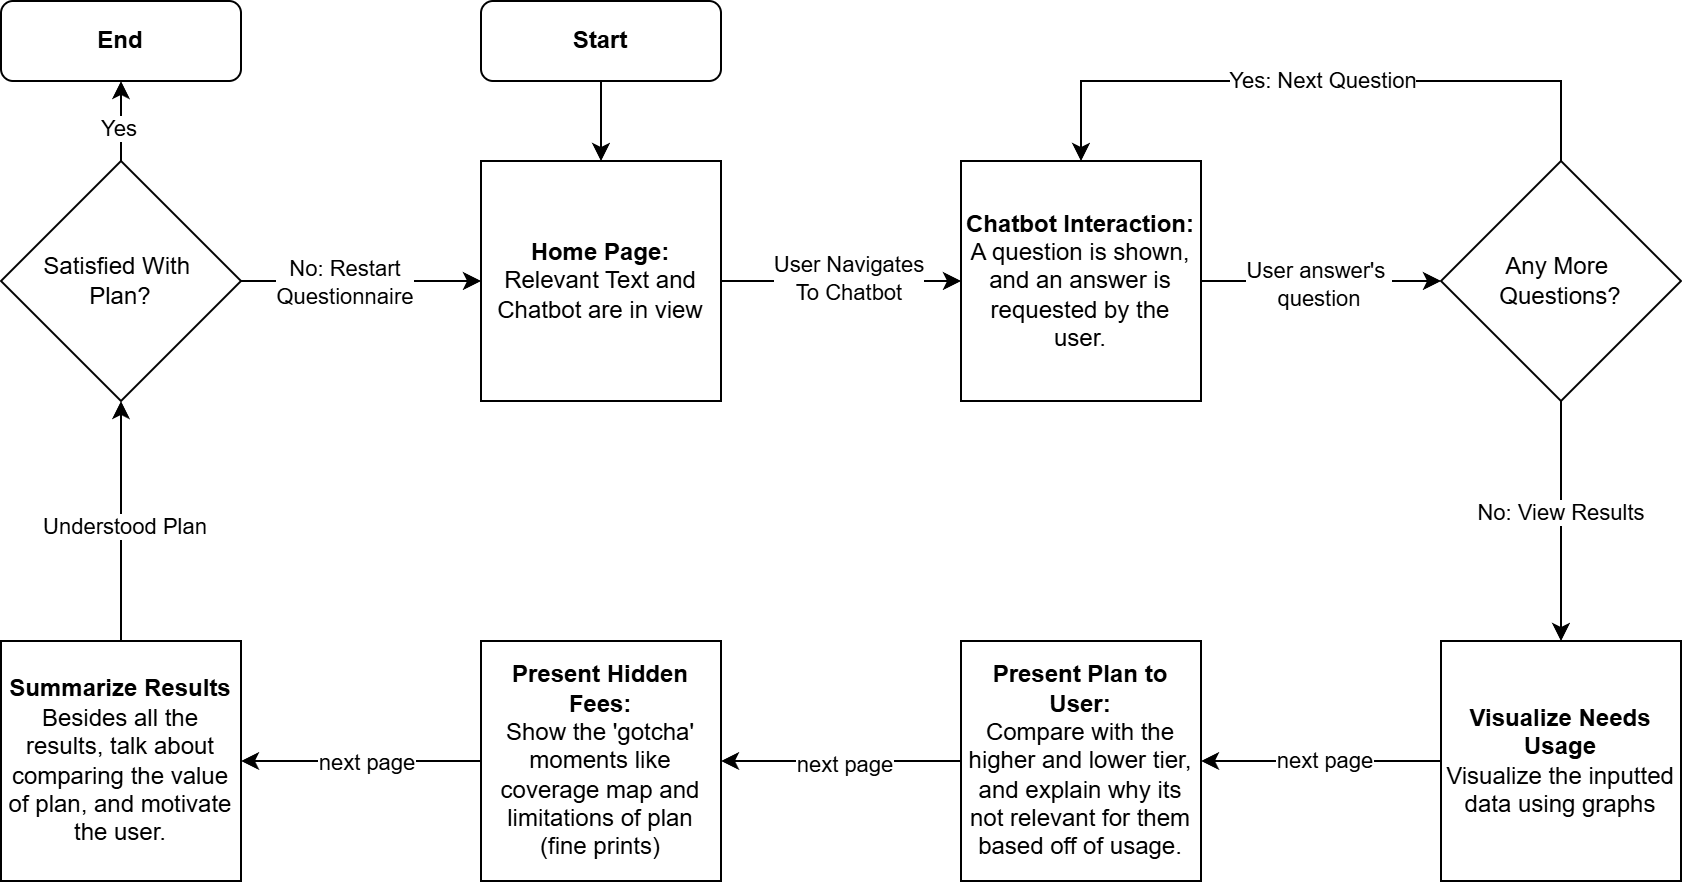
\includegraphics[width=1\linewidth]{FlowChart_357.png}
    \caption{User Flow Diagram of interacting with a Chatbot}
    \label{fig:user flow}
\end{figure}
\subsection{Important Links:}
\begin{itemize}
    \item \href{https://www.figma.com/design/3bhrHSNXqwNiBmlOOrQMPk/SOEN357_Project?node-id=0-1&t=nTcesERC59Hllvib-1}{Figma URL (Clickable)}
    \item \href{https://github.com/briantkatch/357-my-little-chomsky}{GitHub URL (Source Code)}
    \item \href{https://page.joonbot.com/4d81814c-8f84-489a-9956-159db0459389}{Prototype (Try it out now!)}
\end{itemize}
\subsection{Wireframes}
\begin{figure}[H]
    \centering
    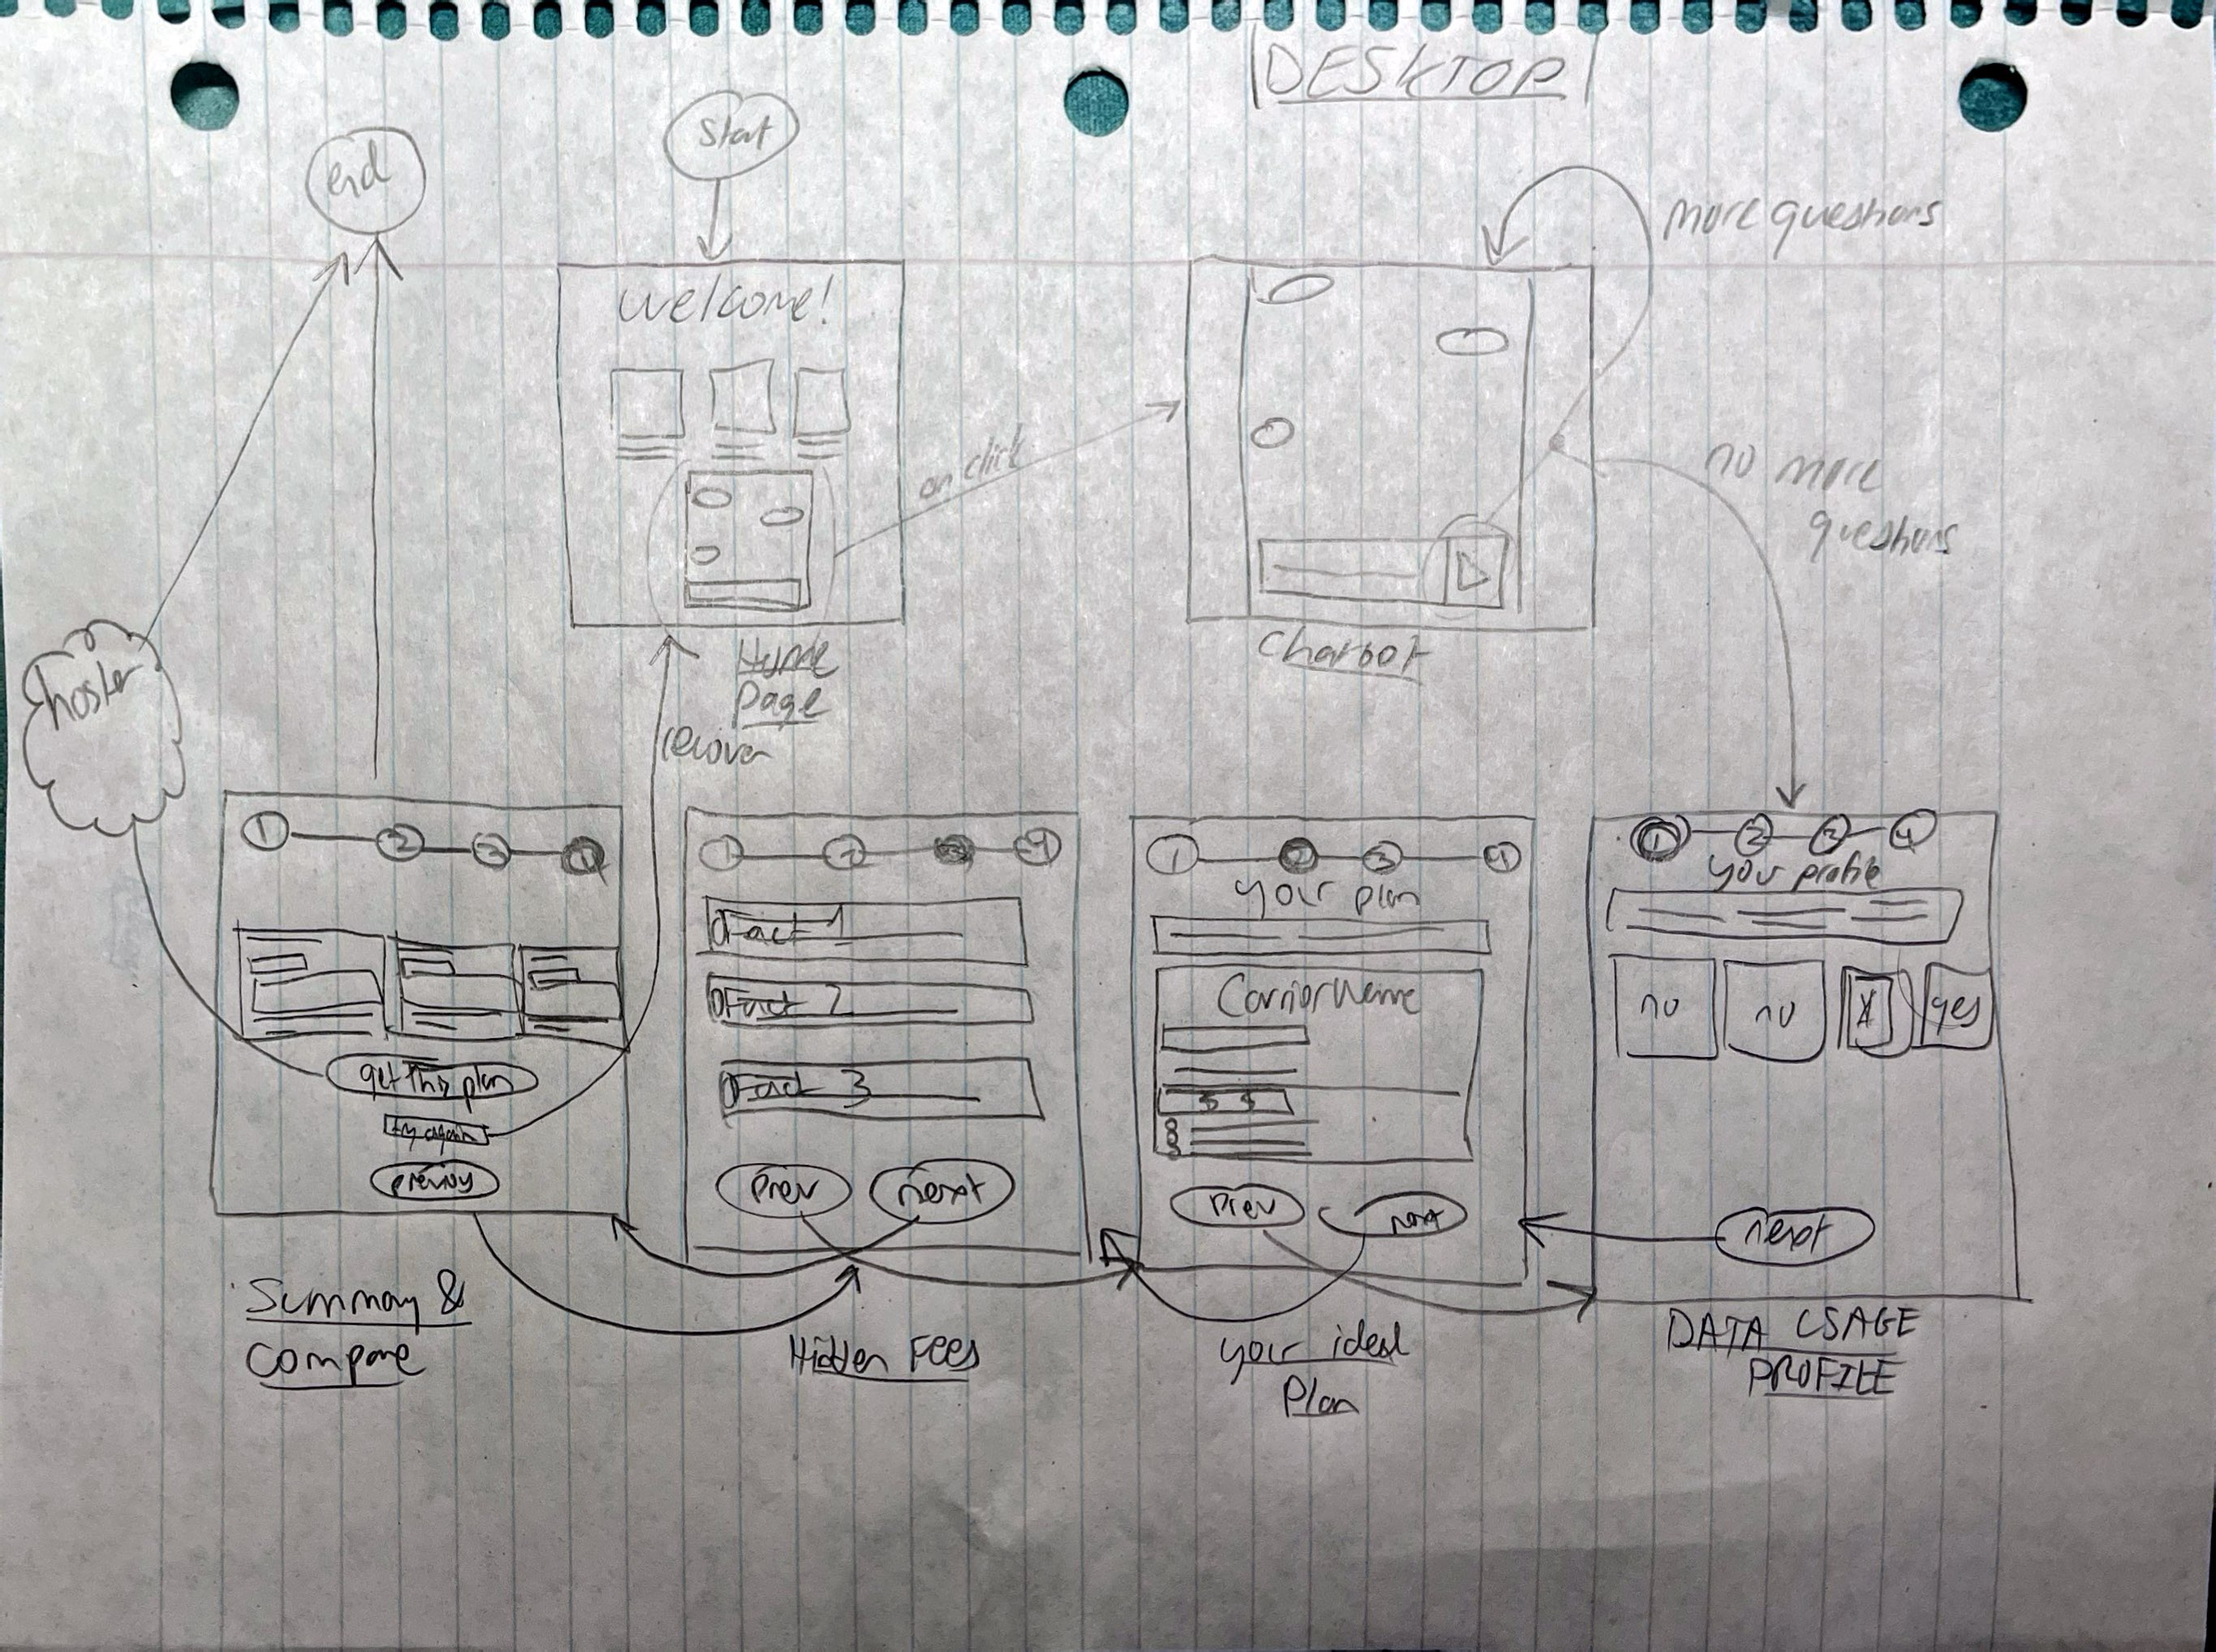
\includegraphics[width=1\linewidth]{Desktop_wireframe.jpg}
    \caption{Wireframe of desktop view}
    \label{fig:user flow}
\end{figure}
\begin{figure}[H]
    \centering
    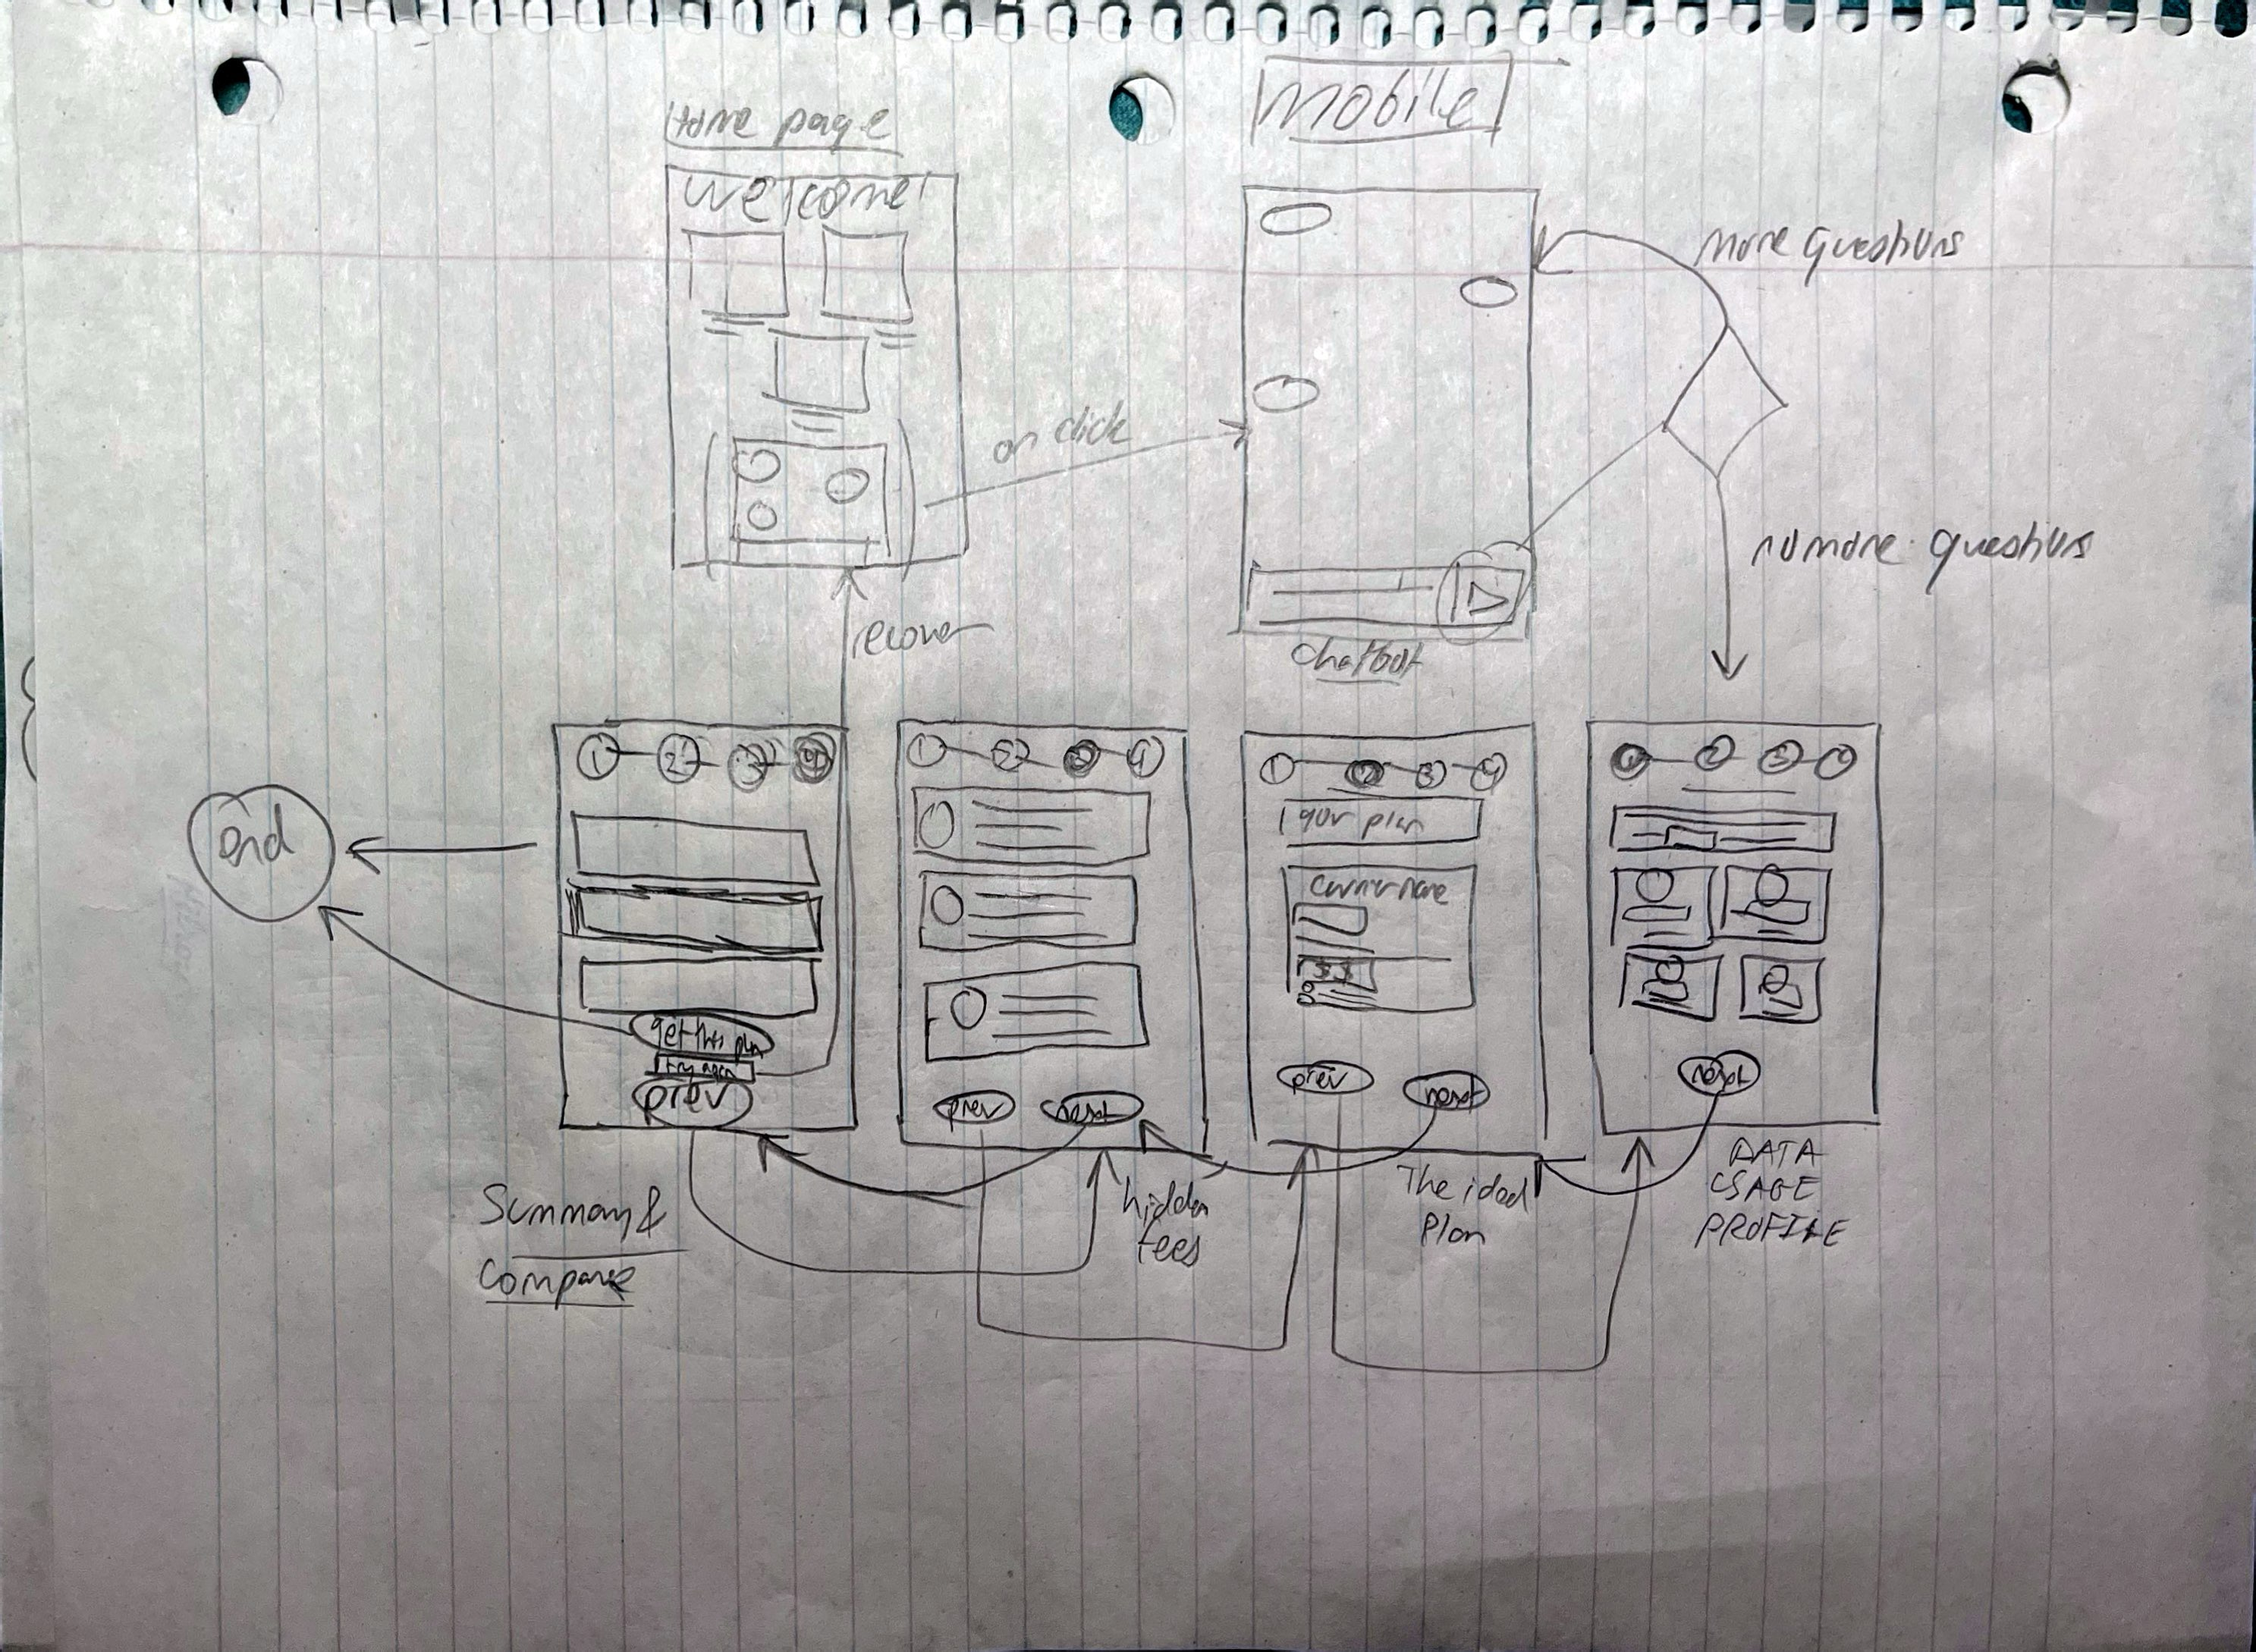
\includegraphics[width=1\linewidth]{Mobile_Wireframe.jpg}
    \caption{Wireframe of mobile view}
    \label{fig:user flow}
\end{figure}
\subsection{Mockups - Desktop}
\begin{figure}[H]
    \centering
    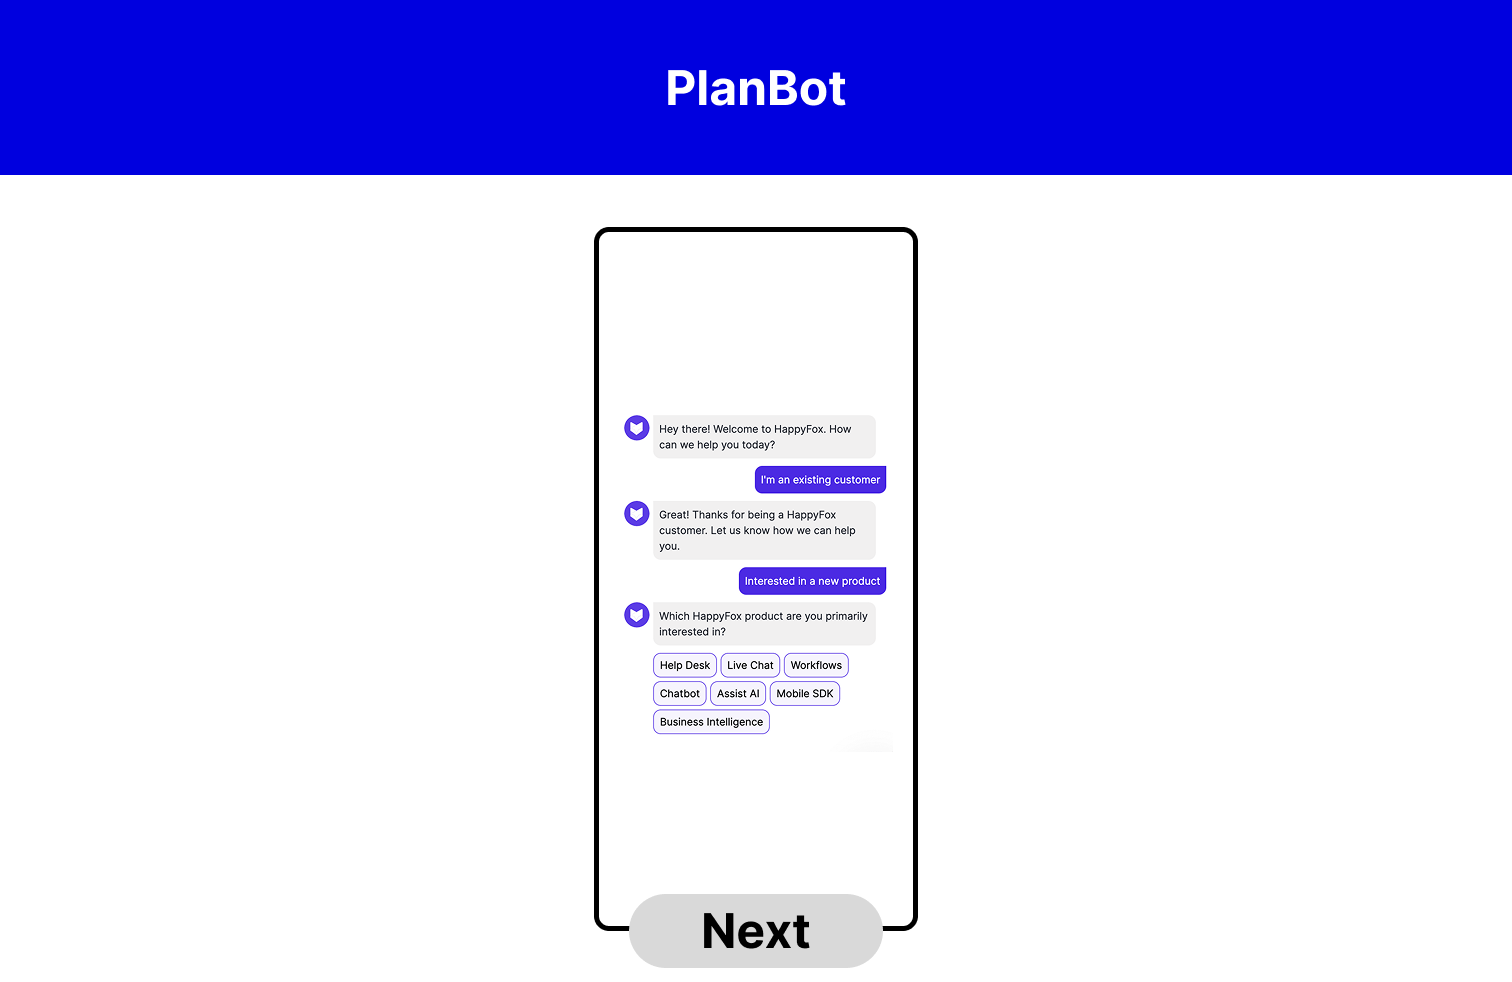
\includegraphics[width=1\linewidth]{Desktop/Chatbot - DesktopDESKTOP.png}
    \caption{Desktop view of Chatbot}
    \label{fig:user flow}
\end{figure}
\begin{figure}[H]
    \centering
    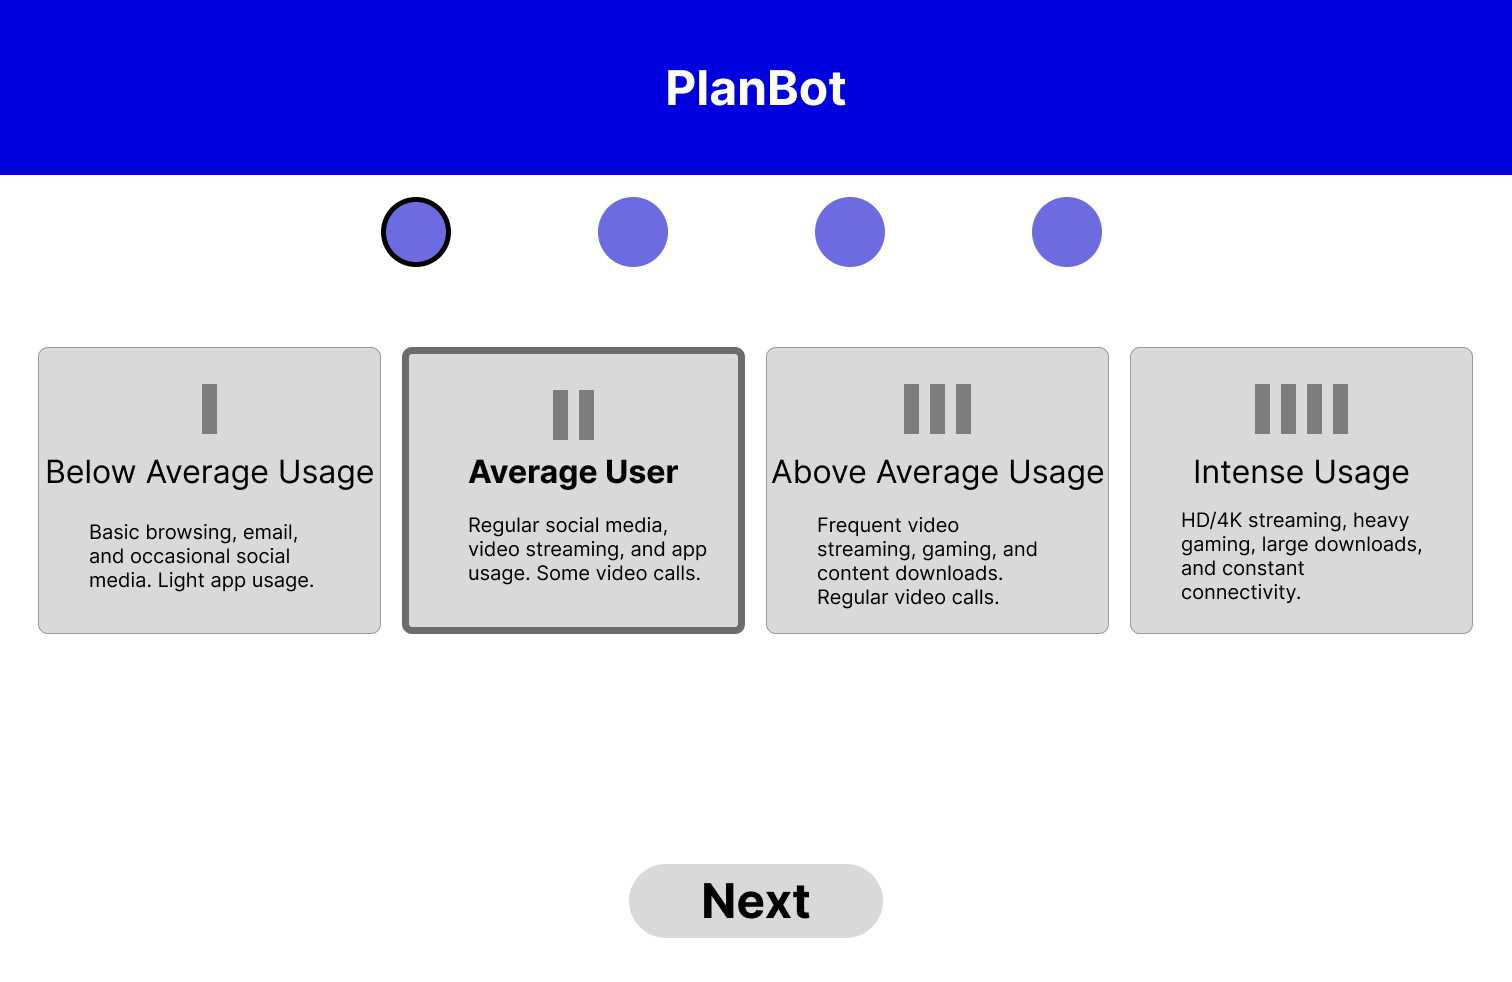
\includegraphics[width=1\linewidth]{Desktop/Data Usage Profile - DesktopDESKTOP.png}
    \caption{Desktop view of Chatbot}
    \label{fig:user flow}
\end{figure}
\begin{figure}[H]
    \centering
    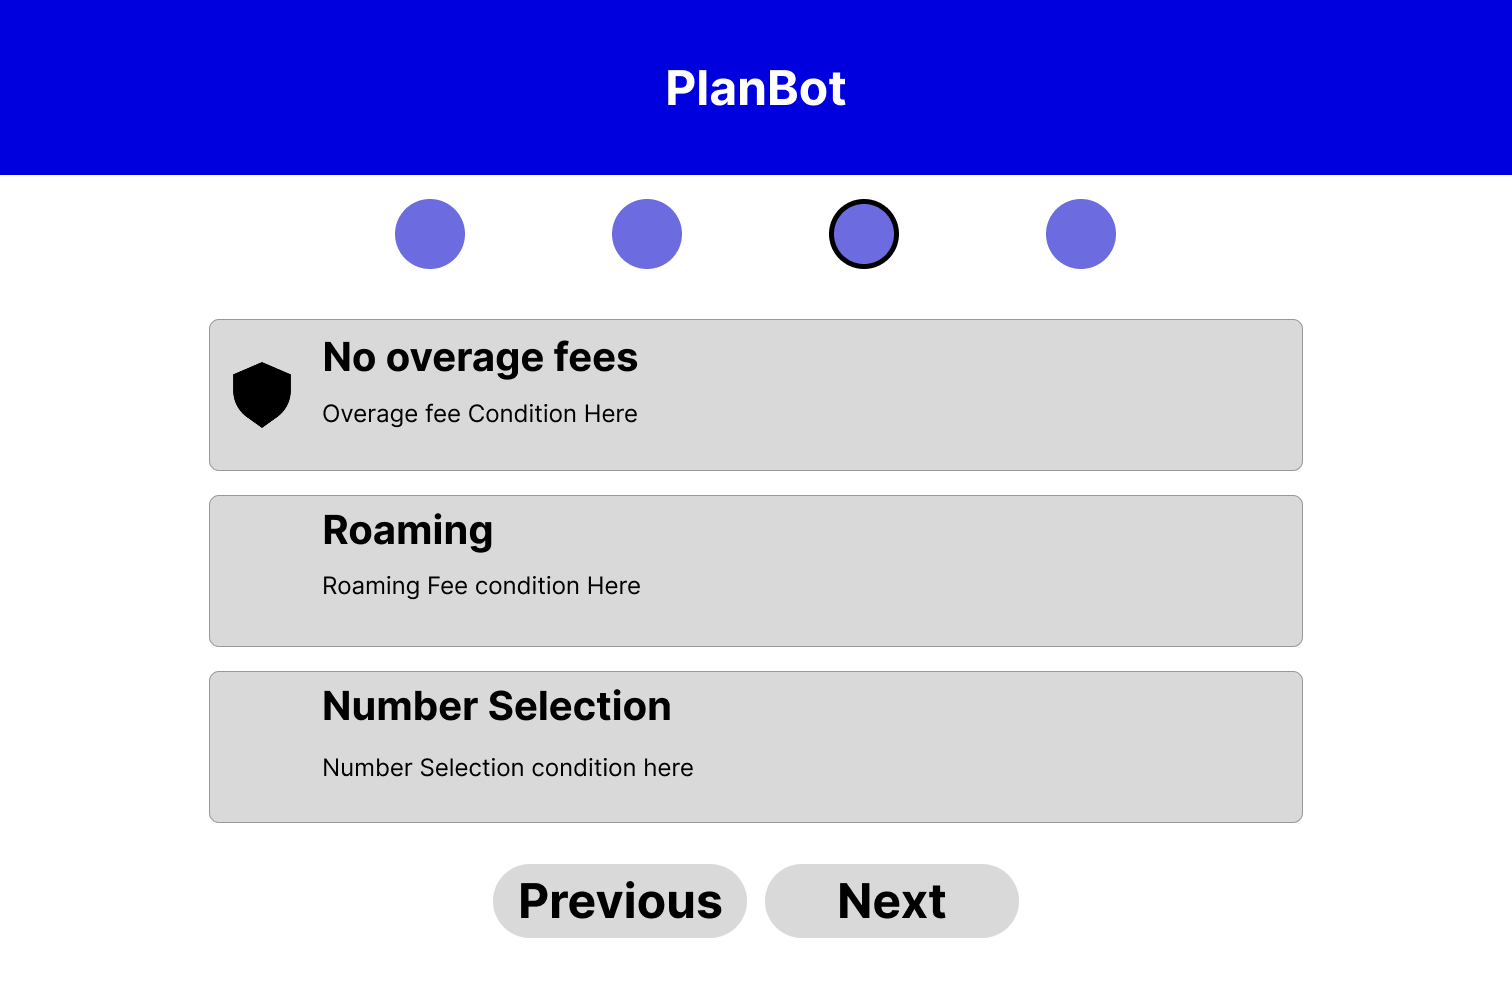
\includegraphics[width=1\linewidth]{Desktop/Hidden Fees - DesktopDESKTOP.png}
    \caption{Desktop view of Data Usage Profile}
    \label{fig:user flow}
\end{figure}
\begin{figure}[H]
    \centering
    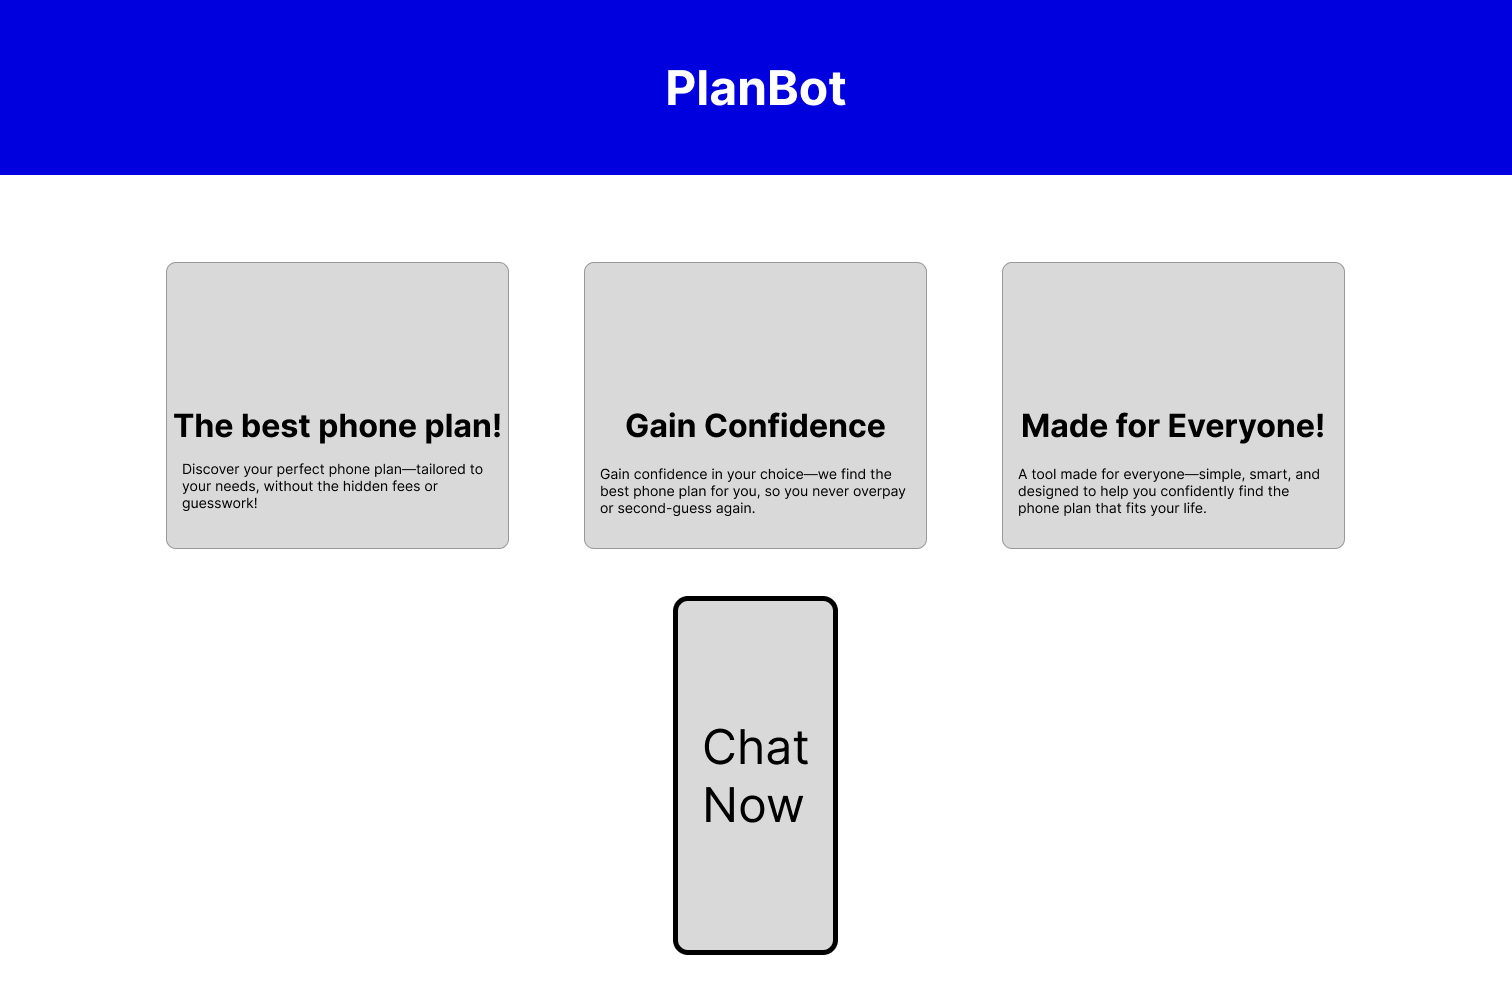
\includegraphics[width=1\linewidth]{Desktop/Home Page - DesktopDESKTOP.png}
    \caption{Desktop view of Hidden Fees}
    \label{fig:user flow}
\end{figure}
\begin{figure}[H]
    \centering
    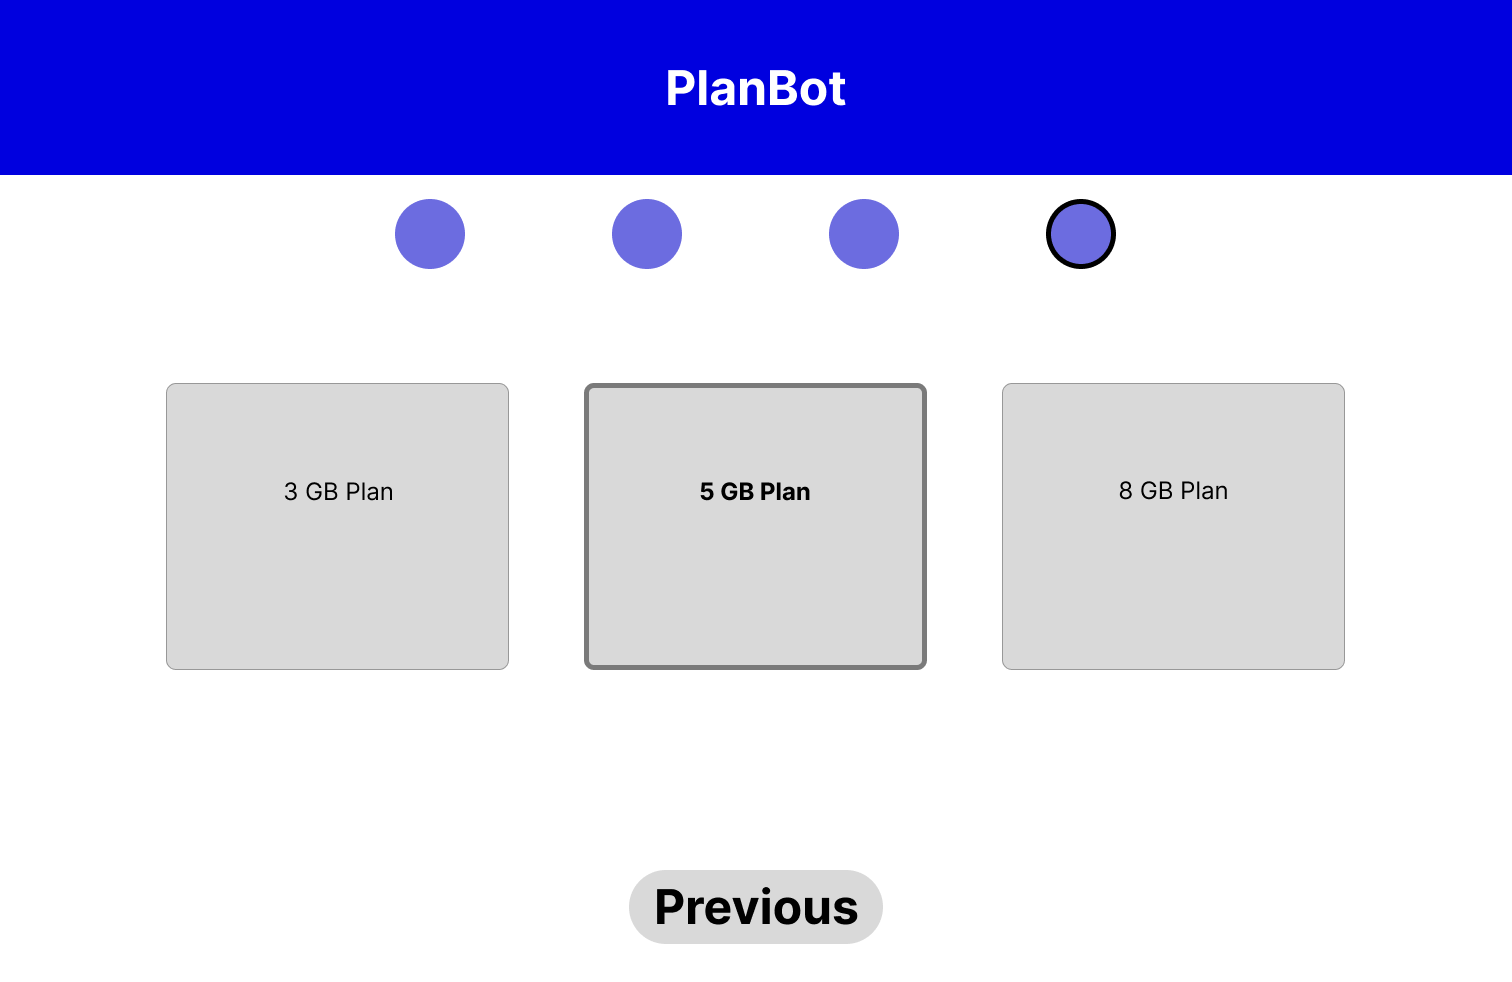
\includegraphics[width=1\linewidth]{Desktop/Summary and Compare - DesktopDESKTOP.png}
    \caption{Desktop view of the main page}
    \label{fig:user flow}
\end{figure}
\begin{figure}[H]
    \centering
    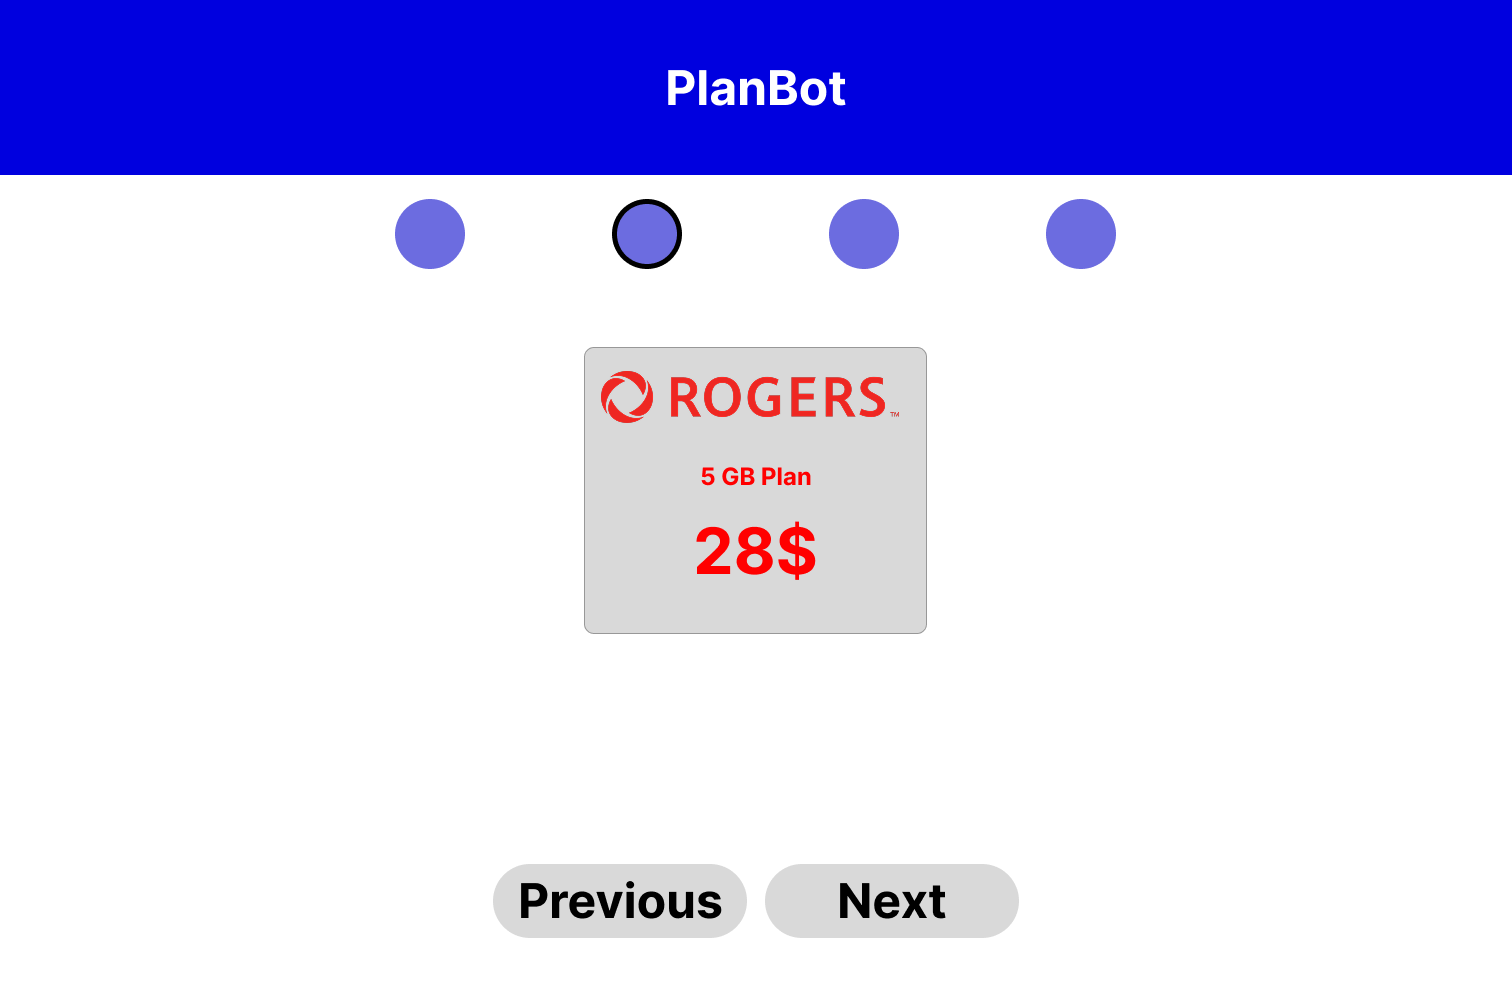
\includegraphics[width=1\linewidth]{Desktop/The Ideal Plan - DesktopDESKTOP.png}
    \caption{Desktop view of Ideal Plan}
    \label{fig:user flow}
\end{figure}
\subsection{Mockups - Mobile}
\begin{figure}[H]
    \centering
    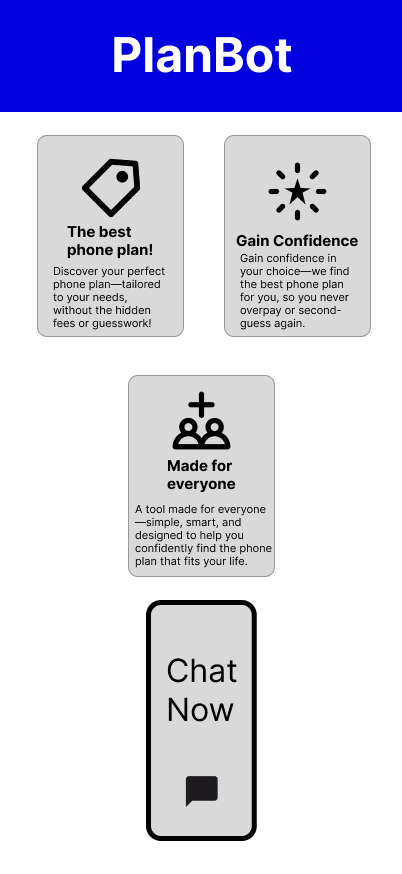
\includegraphics[width=1\linewidth]{Mobile/Group 13MOBILE.png}
    \caption{Mobile view of Home Page}
    \label{fig:user flow}
\end{figure}
\begin{figure}[H]
    \centering
    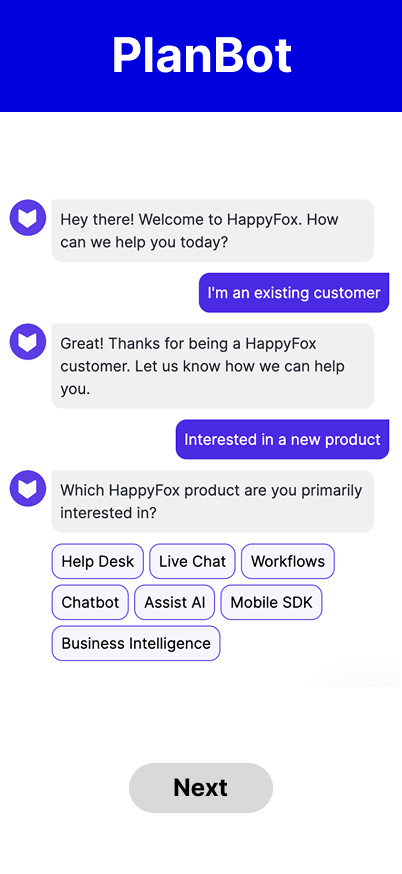
\includegraphics[width=1\linewidth]{Mobile/Group 14MOBILE.png}
    \caption{Mobile view of Chatbot}
    \label{fig:user flow}
\end{figure}
\begin{figure}[H]
    \centering
    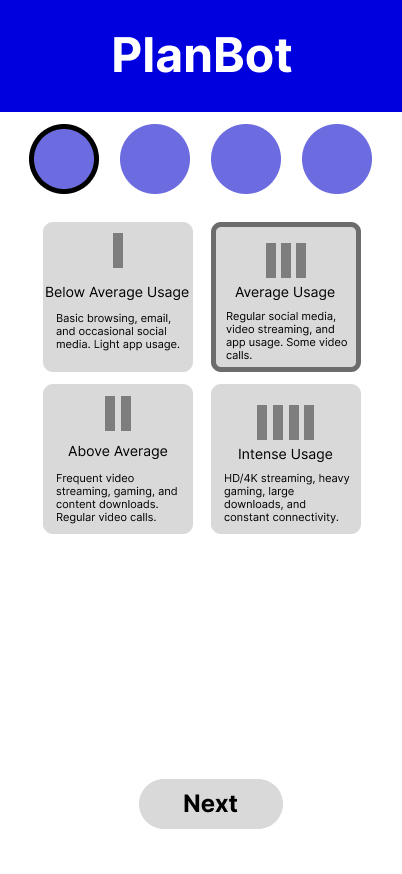
\includegraphics[width=1\linewidth]{Mobile/Group 15MOBILE.png}
    \caption{Mobile view of data usage profile}
    \label{fig:user flow}
\end{figure}
\begin{figure}[H]
    \centering
    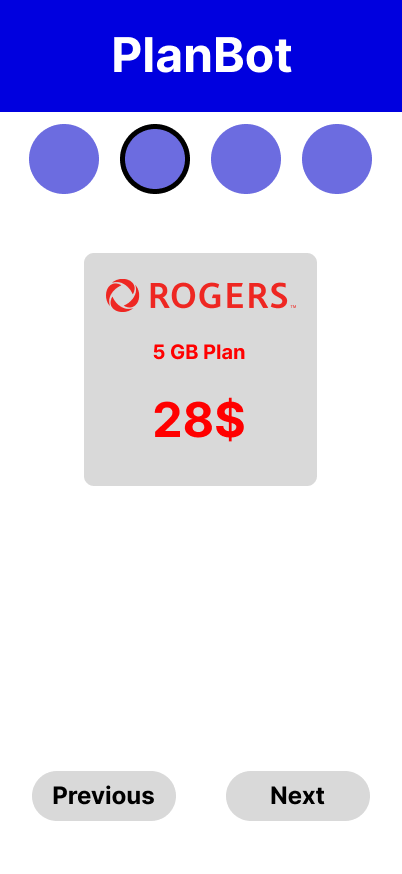
\includegraphics[width=1\linewidth]{Mobile/Group 16MOBILE.png}
    \caption{Mobile view of Home Page}
    \label{fig:user flow}
\end{figure}
\begin{figure}[H]
    \centering
    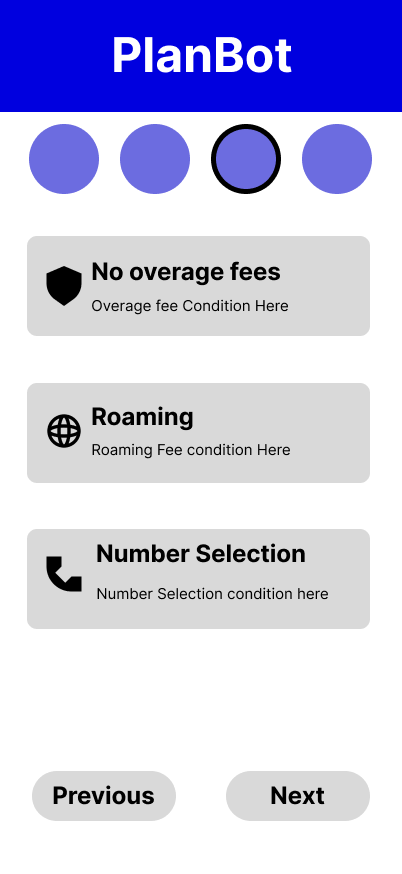
\includegraphics[width=1\linewidth]{Mobile/Group 17MOBILE.png}
    \caption{Mobile view of Hidden Fees}
    \label{fig:user flow}
\end{figure}
\begin{figure}[H]
    \centering
    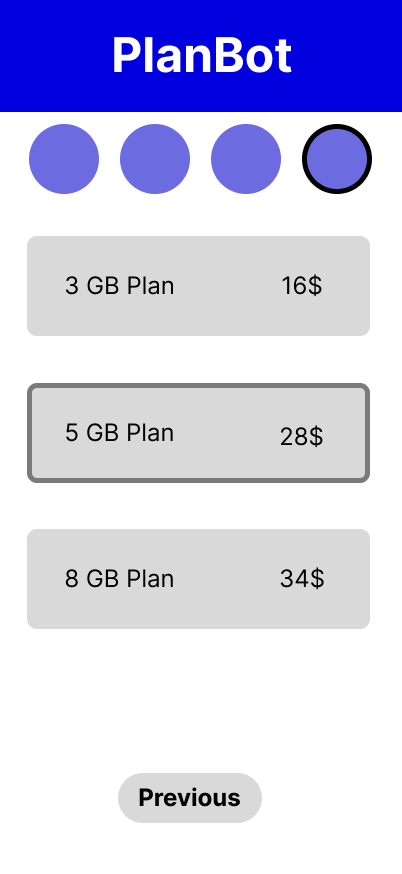
\includegraphics[width=1\linewidth]{Mobile/Group 18MOBILE.png}
    \caption{Mobile view of The Ideal Plan }
    \label{fig:user flow}
\end{figure}
\subsection{JoonBot}
\begin{figure}[H]
    \centering
    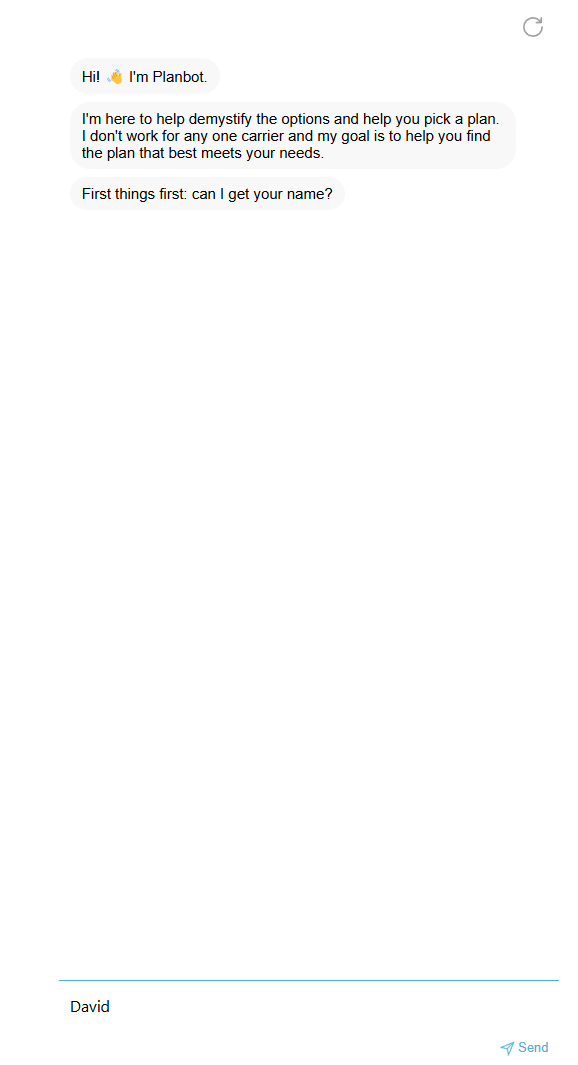
\includegraphics[width=1\linewidth]{joonbotChat.png}
    \caption{Joonbot Chat}
    \label{fig:user flow}
\end{figure}
\begin{figure}[H]
    \centering
    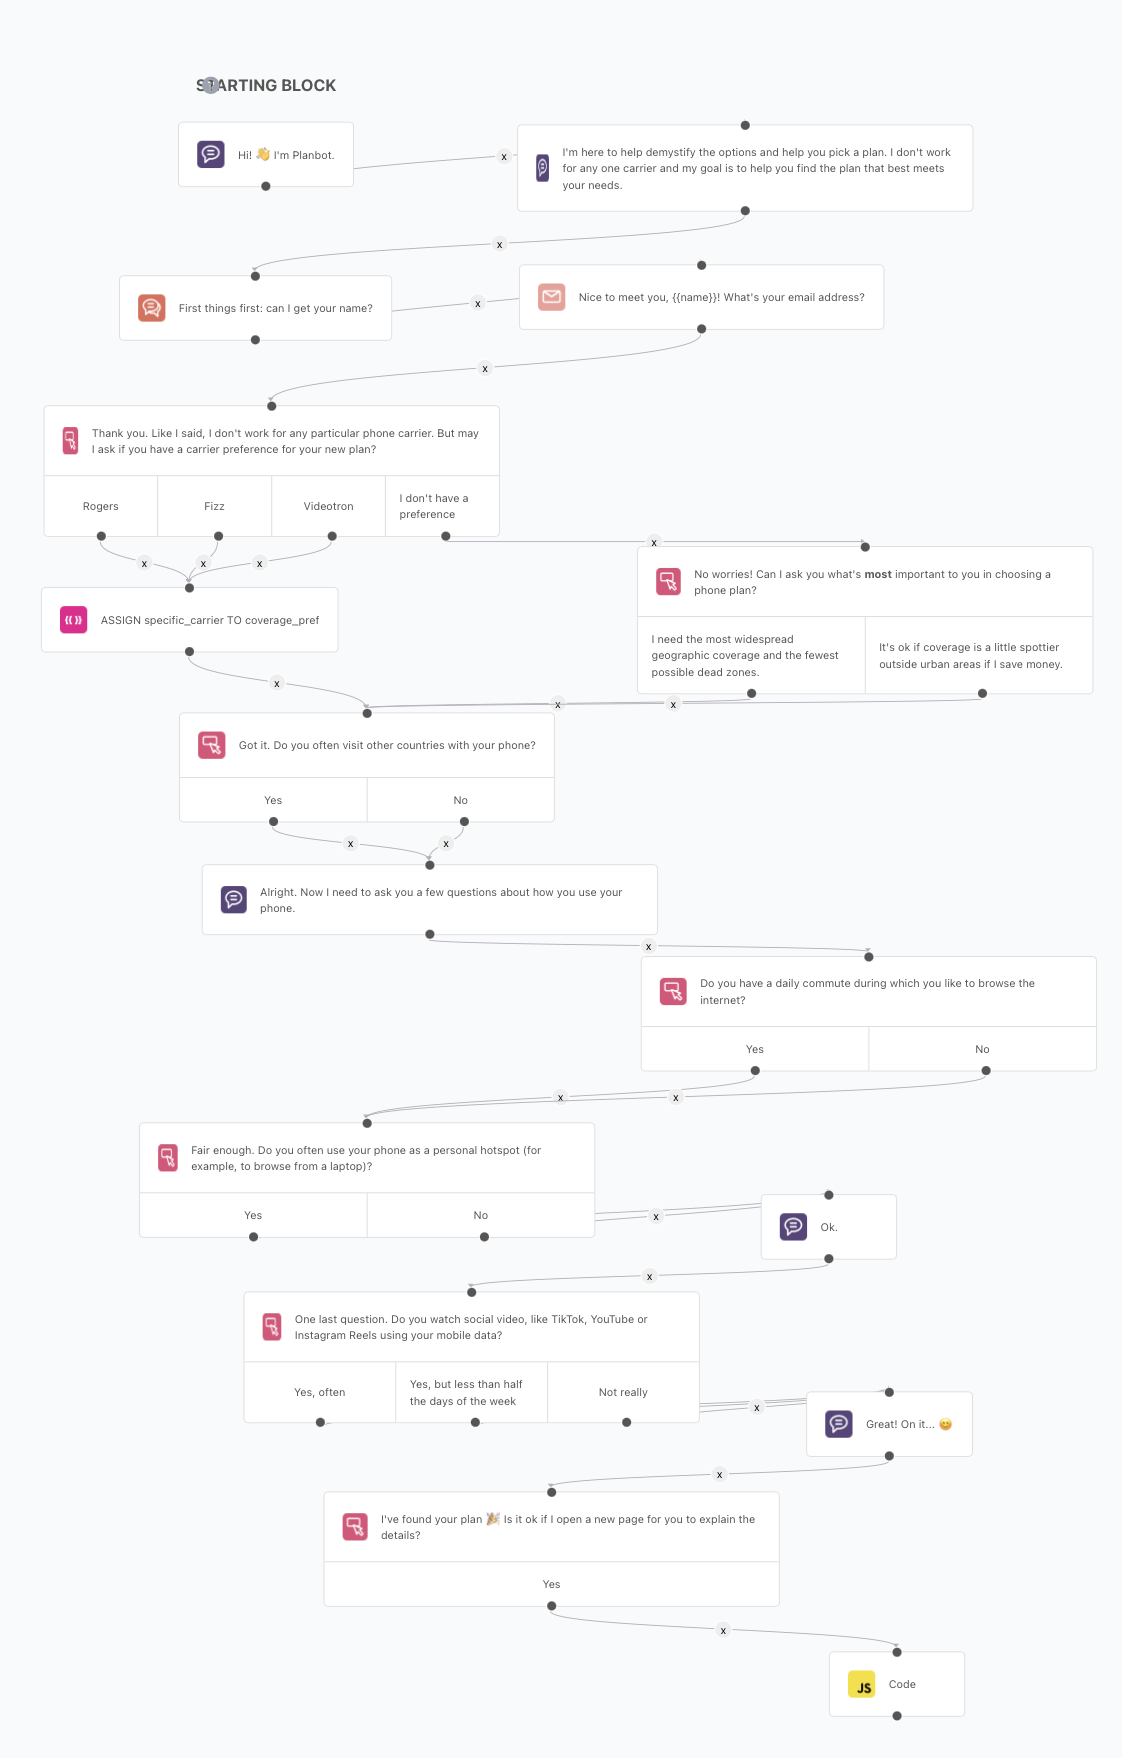
\includegraphics[width=1\linewidth]{joonbot-flow.png}
    \caption{Joonbot Flow}
    \label{fig:user flow}
\end{figure}
\subsection{Prototype V1}
\begin{figure}[H]
    \centering
    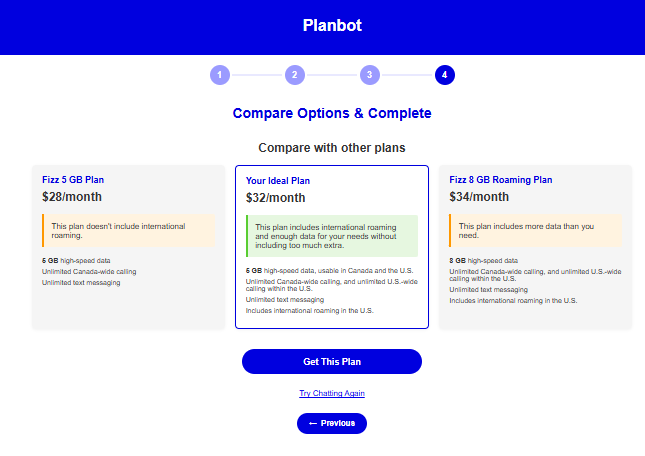
\includegraphics[width=1\linewidth]{Prototype V1/compare options.png}
    \caption{Prototype View of Comparing Phone Plan Options}
    \label{fig:user flow}
\end{figure}
\begin{figure}[H]
    \centering
    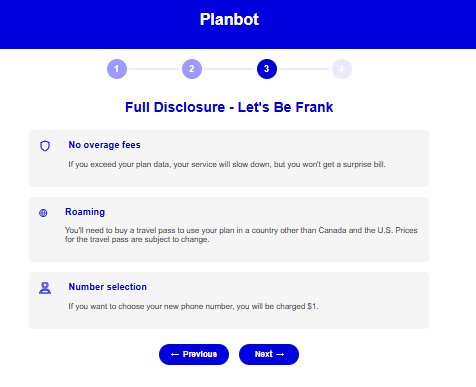
\includegraphics[width=1\linewidth]{Prototype V1/Hidden Fees.png}
    \caption{Prototype View of Hidden Fees page}
    \label{fig:user flow}
\end{figure}
\begin{figure}[H]
    \centering
    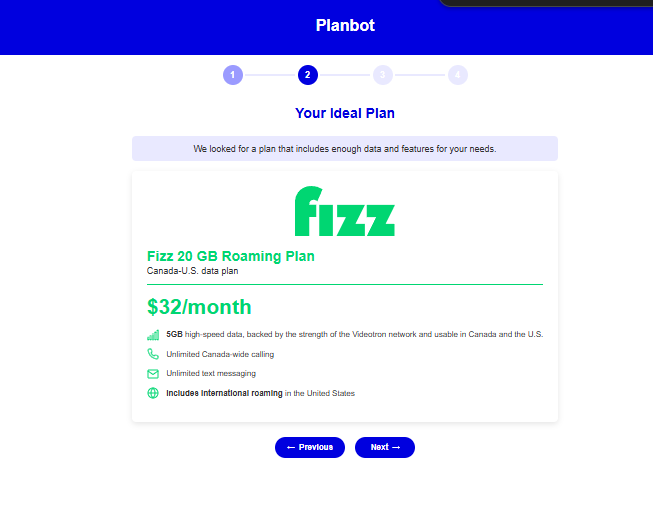
\includegraphics[width=1\linewidth]{Prototype V1/IdealPlan.png}
    \caption{Prototype View of Ideal Plan Page}
    \label{fig:user flow}
\end{figure}
\begin{figure}[H]
    \centering
    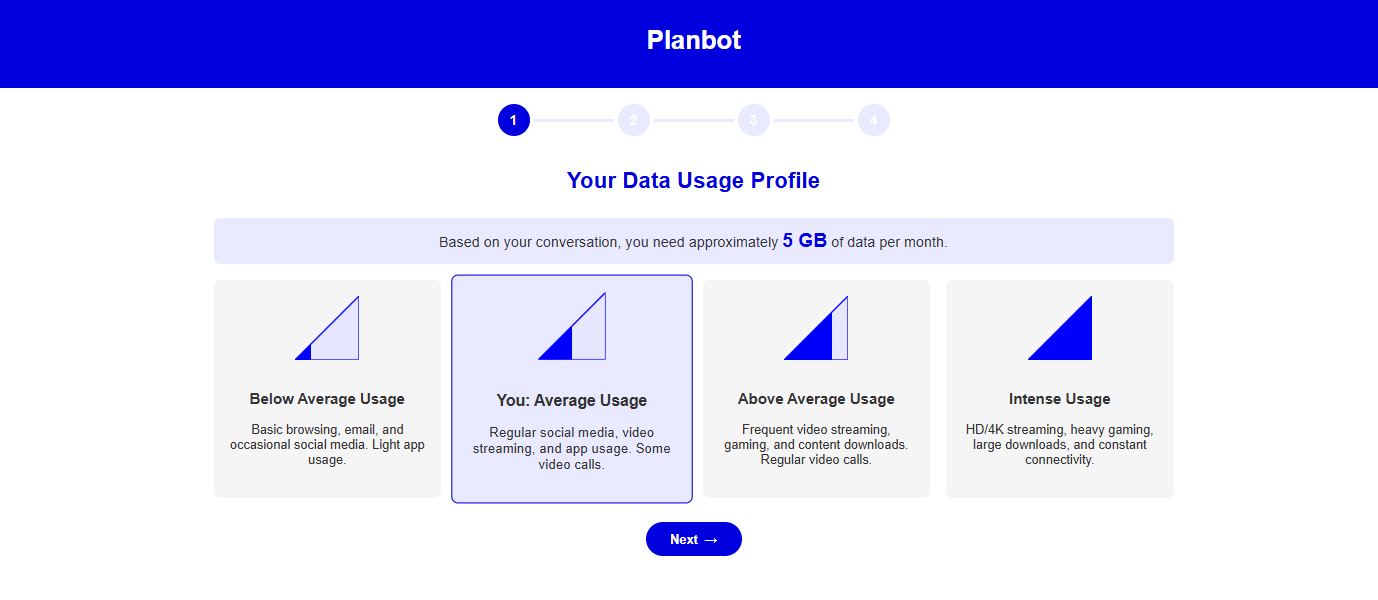
\includegraphics[width=1\linewidth]{Prototype V1/UserNeeds.png}
    \caption{Prototype View of user needs page}
    \label{fig:user flow}
\end{figure}
\subsection{Prototype V2}
\begin{figure}[H]
    \centering
    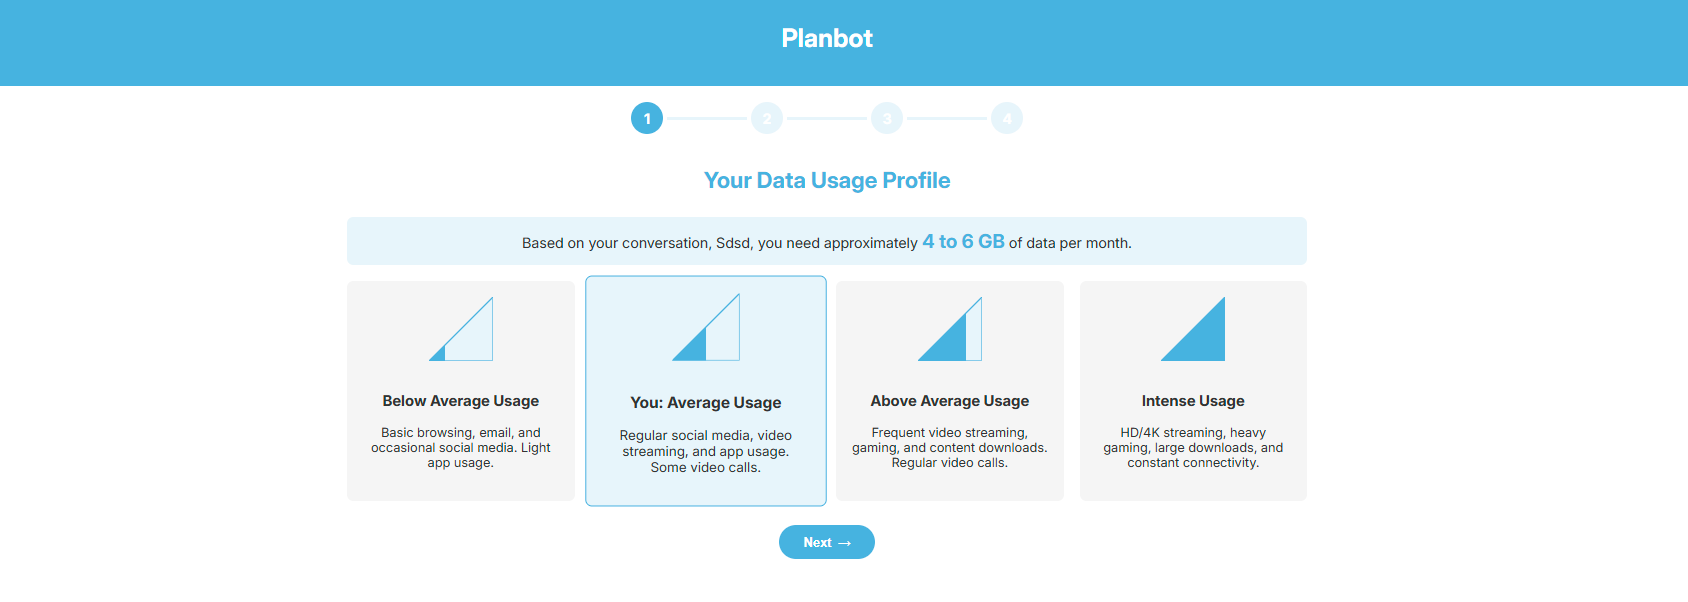
\includegraphics[width=1\linewidth]{Prototype V2/1-357.png}
    \caption{Prototype after refinement of Data Usage Profile}
    \label{fig:user flow}
\end{figure}
\begin{figure}[H]
    \centering
    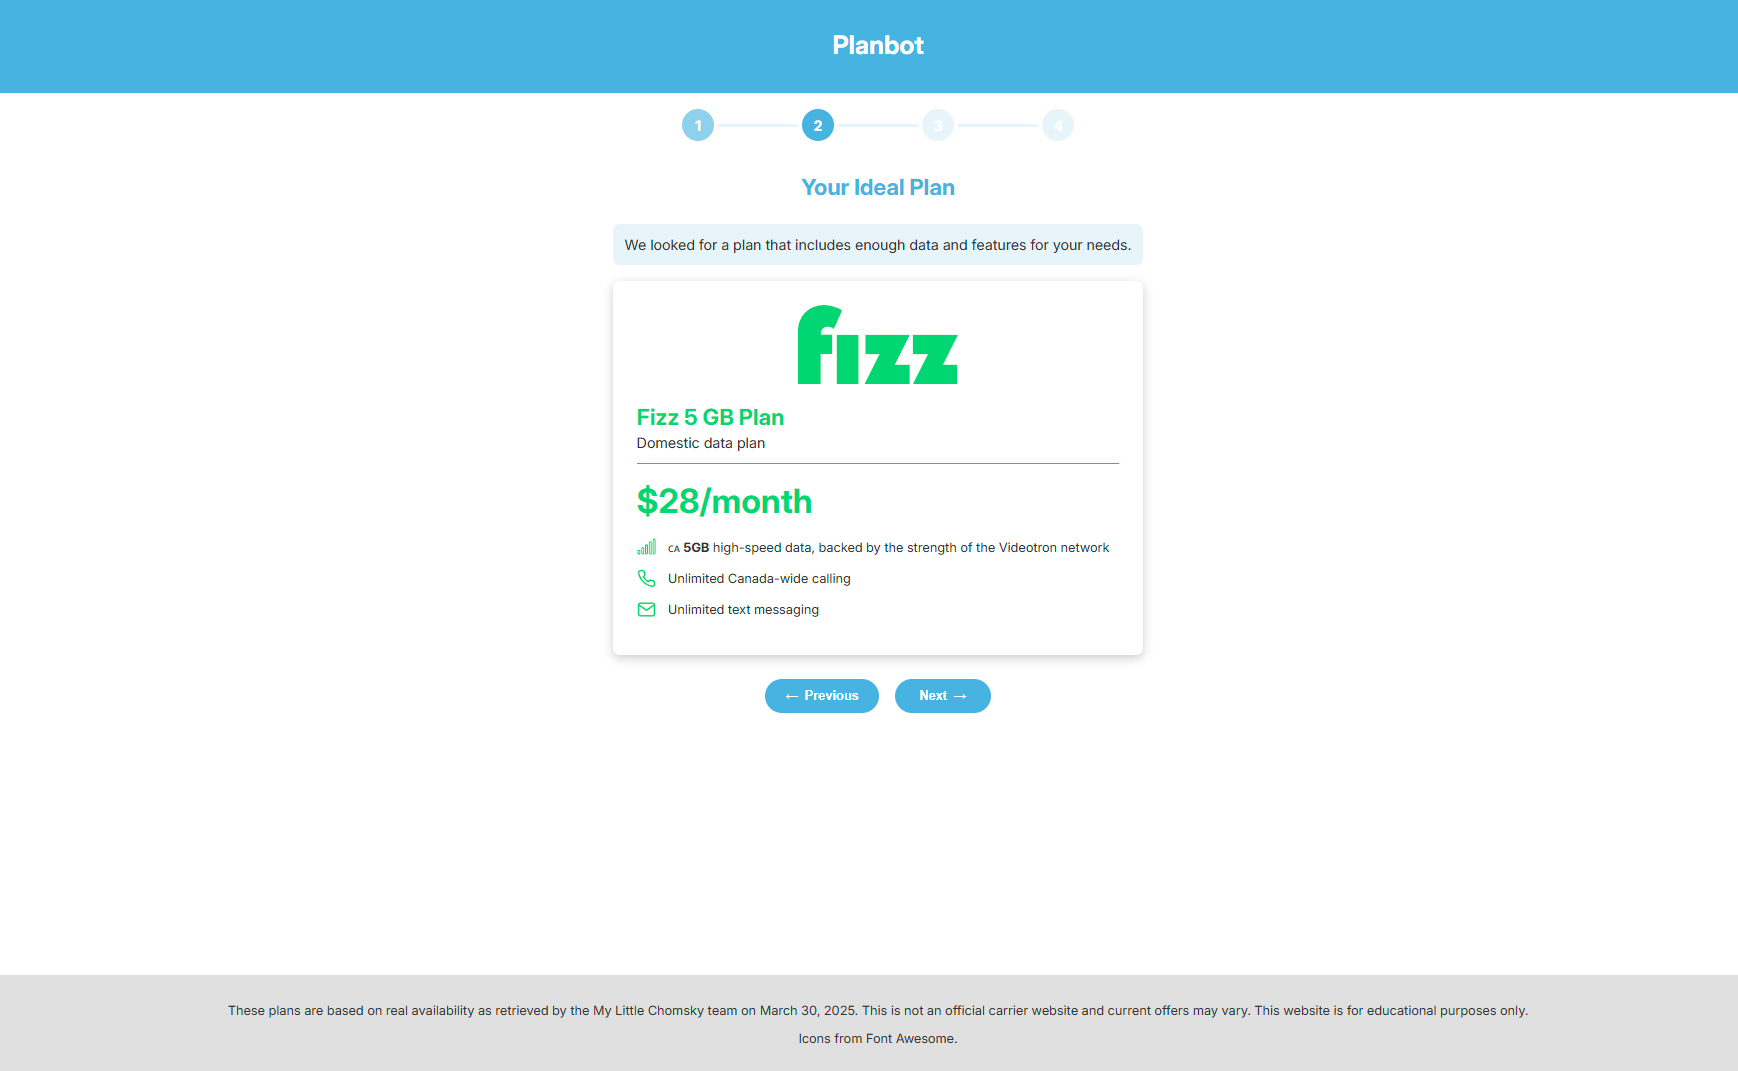
\includegraphics[width=1\linewidth]{Prototype V2/2-357.png}
    \caption{Prototype after refinement of Ideal Plan}
    \label{fig:user flow}
\end{figure}
\begin{figure}[H]
    \centering
    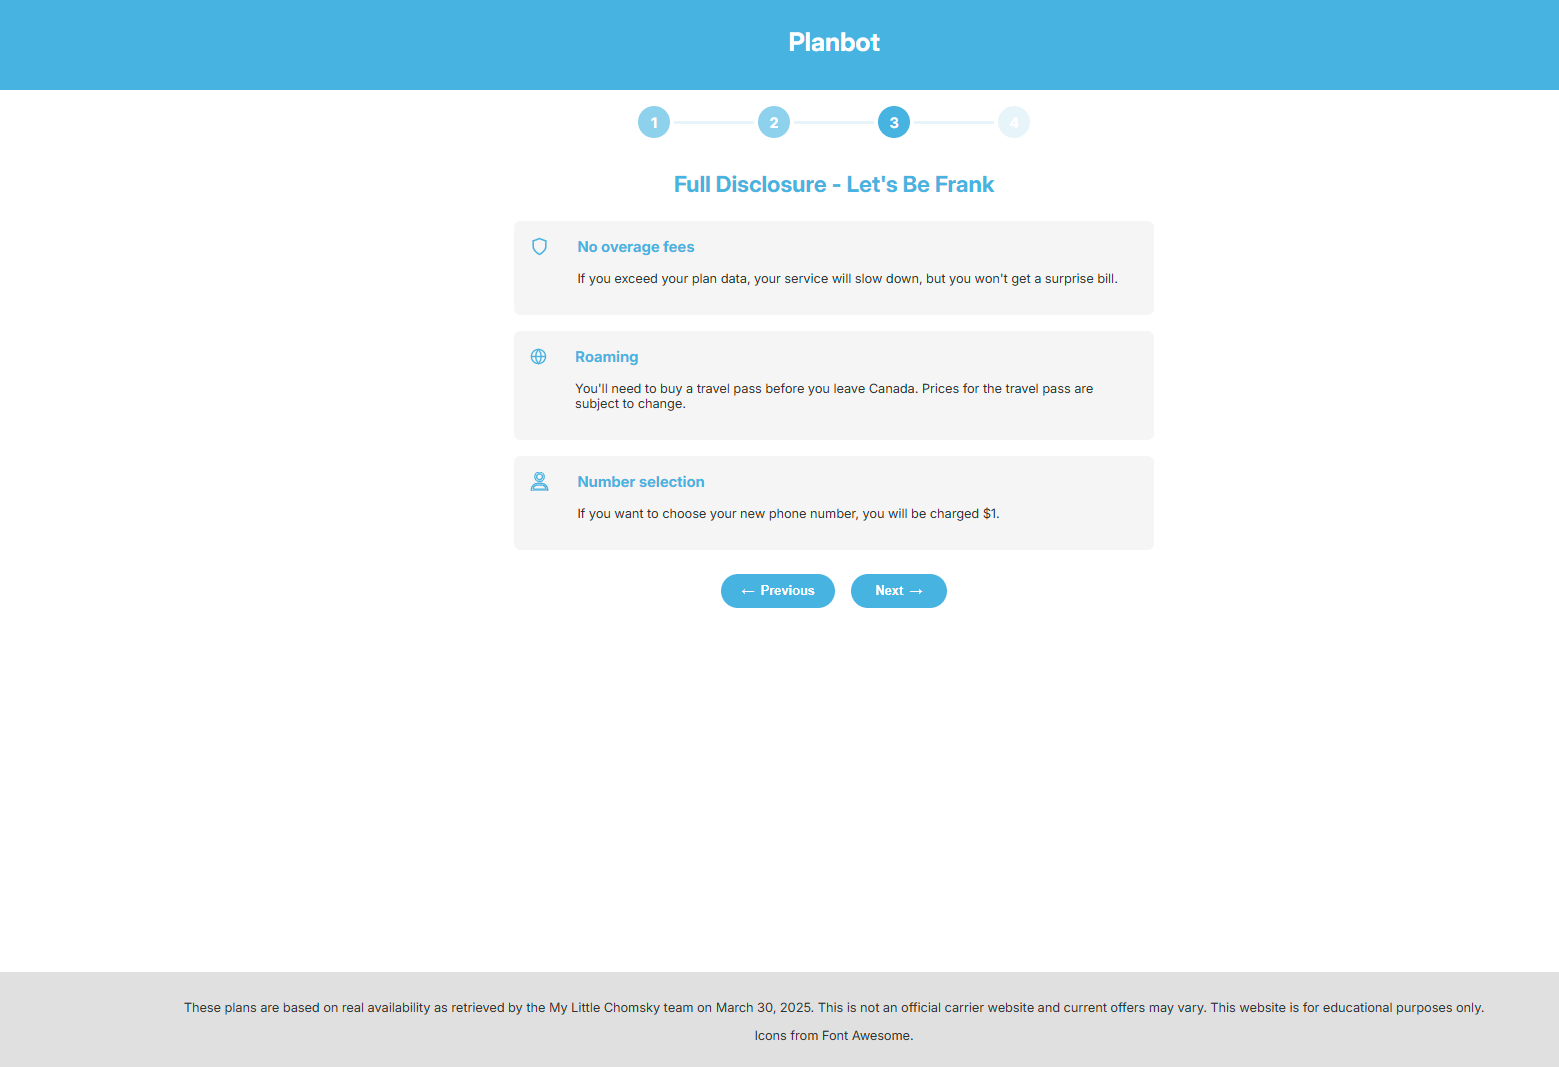
\includegraphics[width=1\linewidth]{Prototype V2/3-357.png}
    \caption{Prototype after refinement of Hidden Fees}
    \label{fig:user flow}
\end{figure}
\begin{figure}[H]
    \centering
    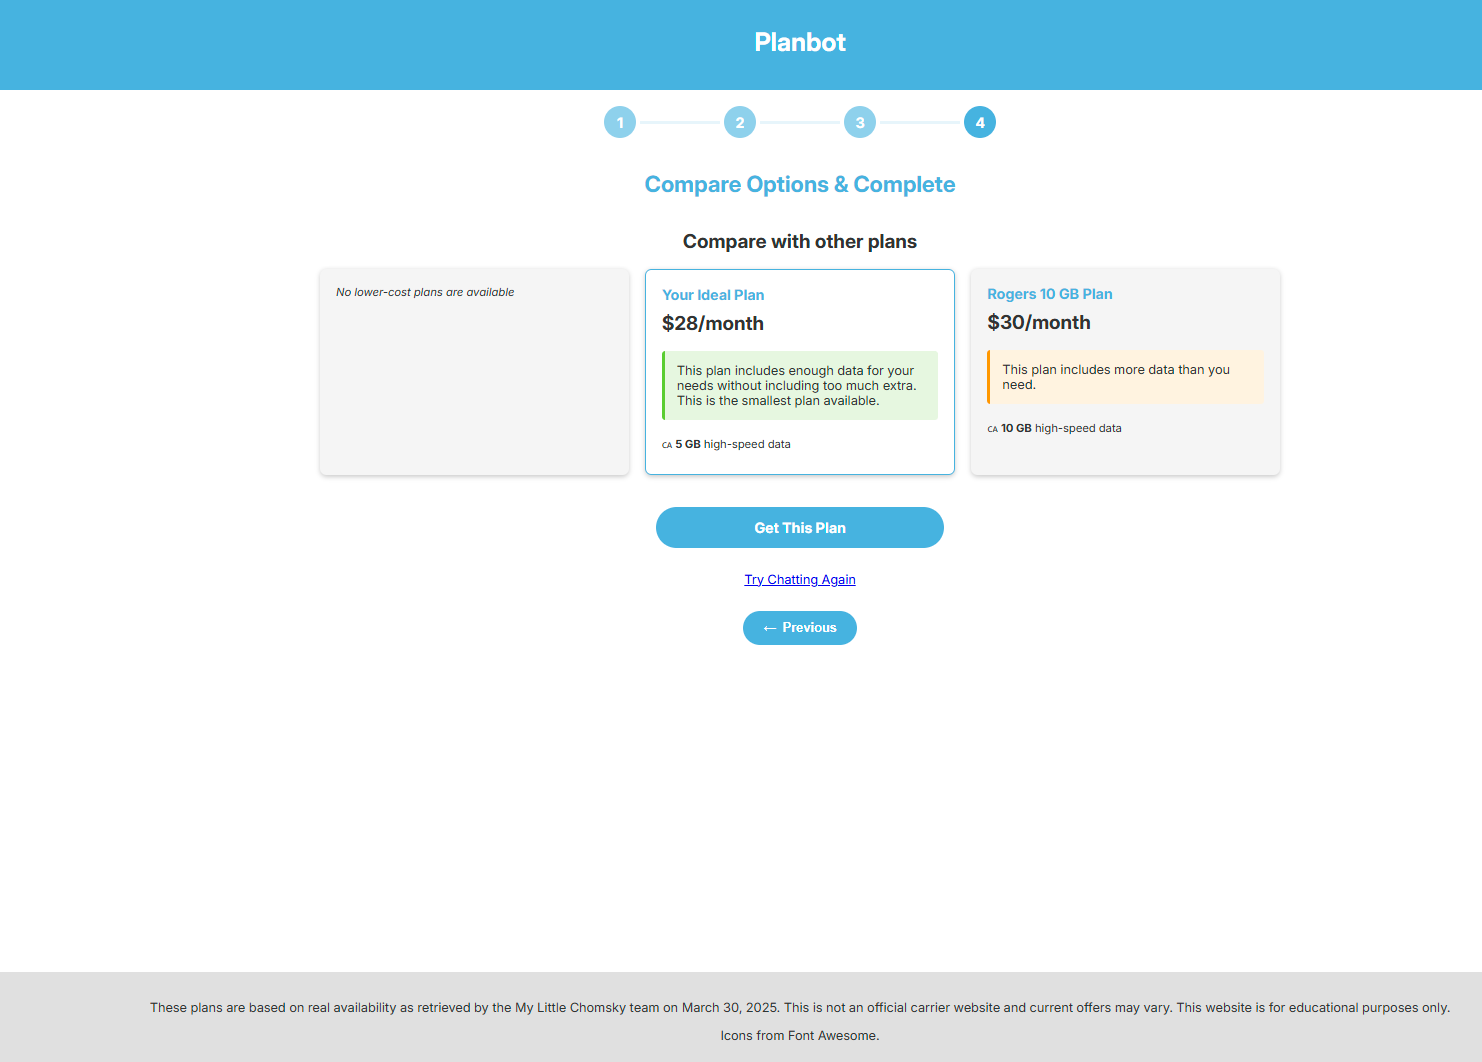
\includegraphics[width=1\linewidth]{Prototype V2/4-357.png}
    \caption{Prototype after refinement of Phone Plan Comparison}
    \label{fig:user flow}
\end{figure}
\subsection{Data Collection Results}
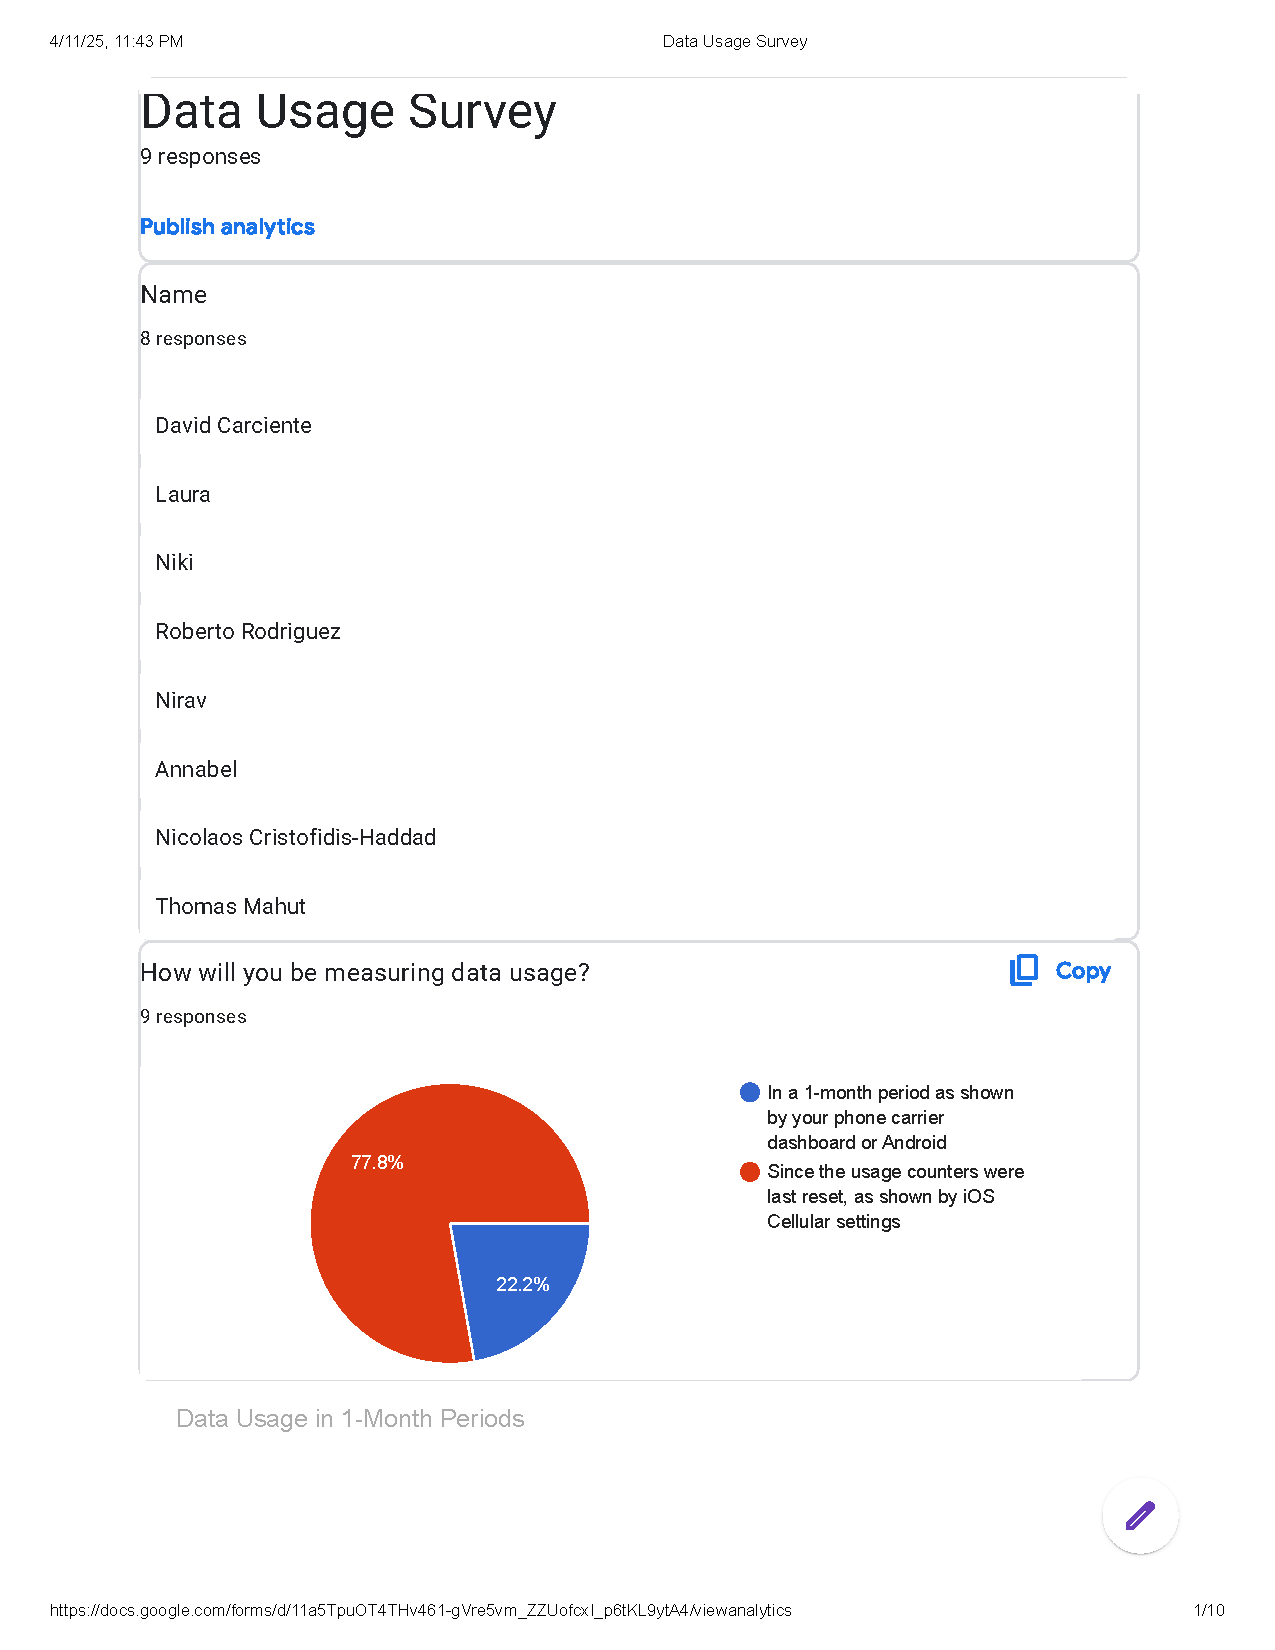
\includepdf[pages=-]{357_Data Usage Survey.pdf}
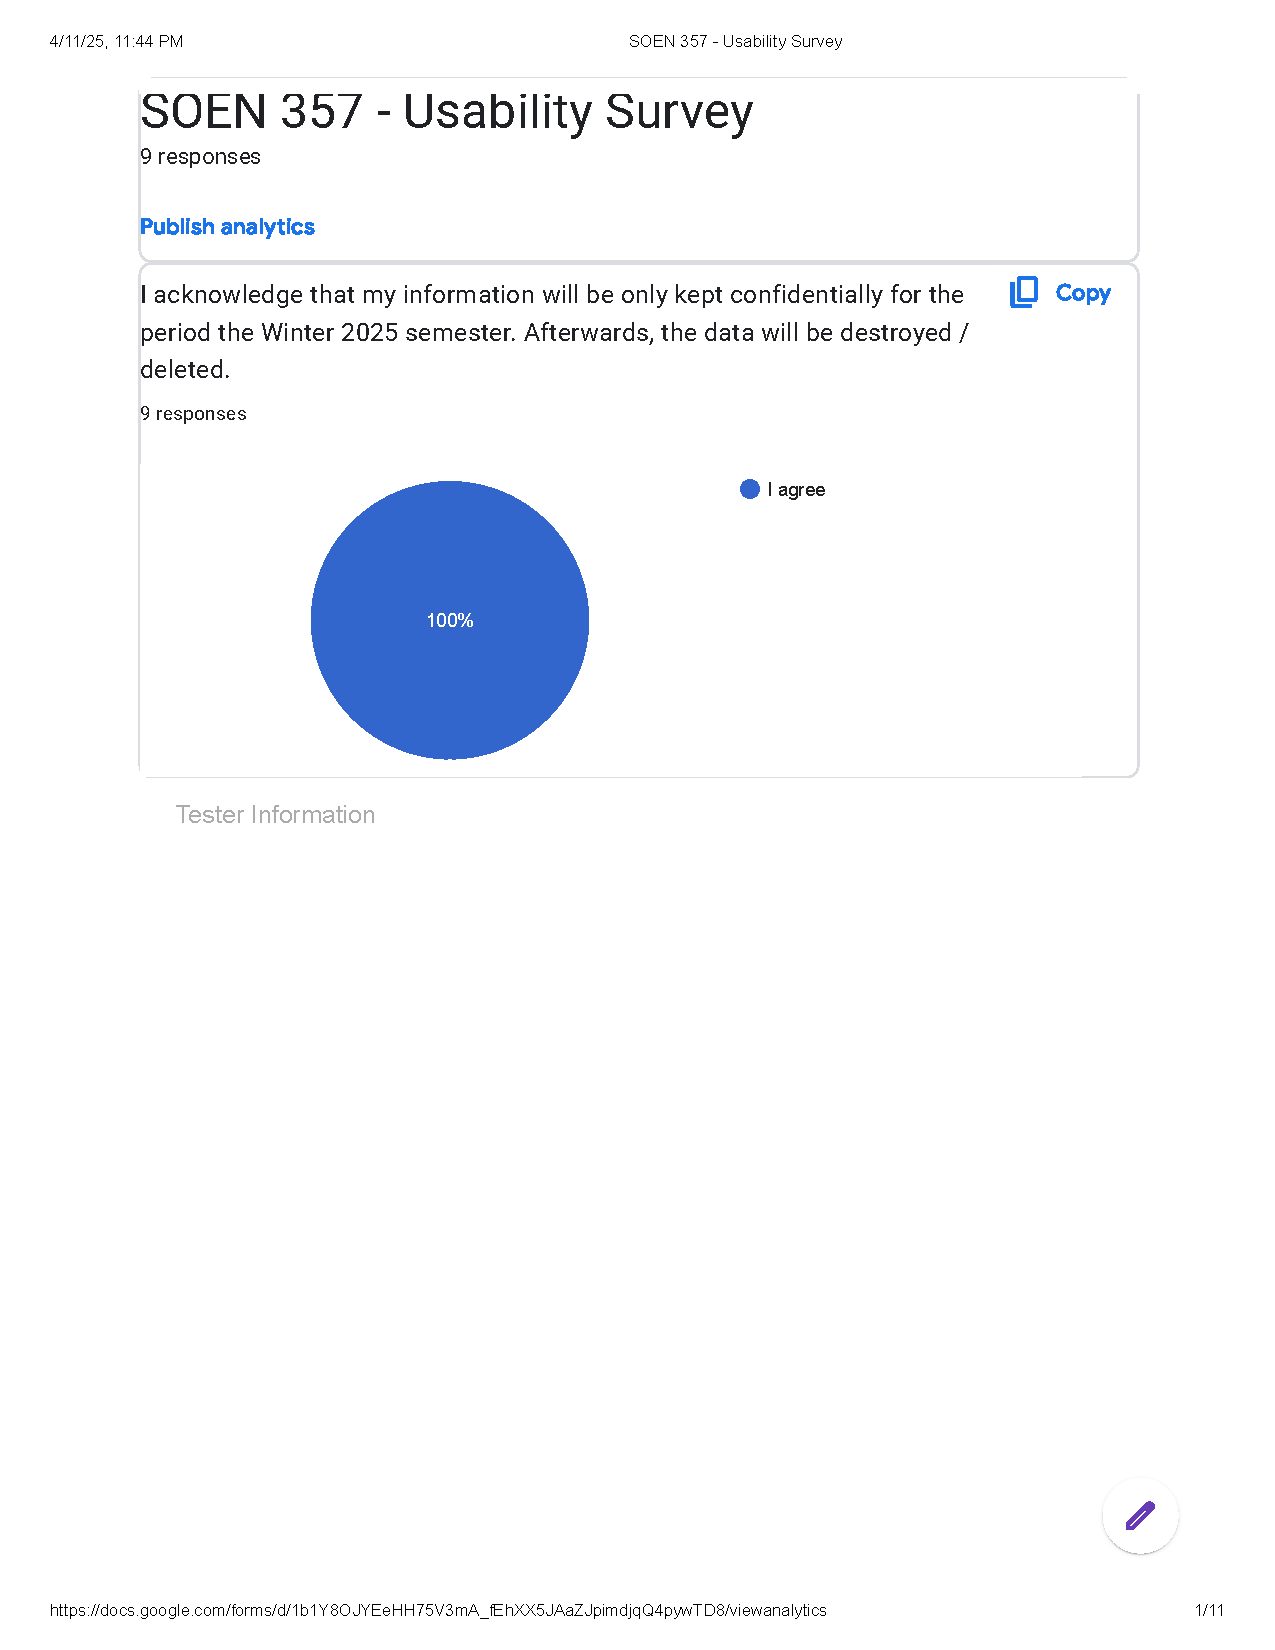
\includepdf[pages=-]{357_SOEN 357 - Usability Survey.pdf}
\end{document}
